\documentclass[twoside,10pt]{book}
\usepackage[amsbb,subscriptcorrection,zswash,mtpcal,mtphrb]{mtpro2}
\usepackage[no-math,cm-default]{fontspec}
\usepackage{xunicode}
\usepackage{xgreek}
\defaultfontfeatures{Mapping=tex-text,Scale=MatchLowercase}
\setmainfont[Mapping=tex-text,Numbers=Lining,Scale=1.0,BoldFont={Minion Pro Bold}]{Minion Pro}
\defaultfontfeatures{Ligatures=TeX}
\font\kefalaio="Minion Pro Bold" at 36pt
\font\ArKef="Minion Pro Bold Italic" at 72pt
\font\OnKef="Times New Roman" at 20pt
\font\OnPar="Minion Pro Bold" at 18pt
\newfontfamily\scfont{Times New Roman}
\usepackage[inner=2.00cm, outer=1.50cm, top=3.00cm, bottom=2.00cm,paperwidth=17cm,paperheight=24cm]{geometry}
\usepackage{amsmath}
\usepackage[amsbb,subscriptcorrection,zswash,mtpcal,mtphrb]{mtpro2}
\usepackage{makeidx}
\usepackage{longtable,xcolor,varwidth}
\usepackage{float}
\usepackage{subfig}
\def\xrwma{cyan!70!black}
\def\xrwmath{cyan}
\usepackage{etoolbox}
\makeatletter
\newif\ifLT@nocaption
\preto\longtable{\LT@nocaptiontrue}
\appto\endlongtable{%
\ifLT@nocaption
\addtocounter{table}{\m@ne}%
\fi}
\preto\LT@caption{%
\noalign{\global\LT@nocaptionfalse}}
\makeatother
\makeindex
\usepackage{tikz,pgfplots}
\usepackage{tkz-euclide,tkz-fct}
\usetikzlibrary{fadings}
\usepackage{wrap-rl}
\usetkzobj{all}
\usepackage{calc}
\usepackage[colorlinks=false, pdfborder={0 0 0}]{hyperref}
\usepackage{cleveref}
\usepackage[framemethod=TikZ]{mdframed}
\definecolor{steelblue}{cmyk}{.7,.278,0,.294}
\definecolor{doc}{cmyk}{1,0.455,0,0.569}
\definecolor{olivedrab}{cmyk}{0.25,0,0.75,0.44}
\usepackage{capt-of}
\usepackage{titletoc}
\usepackage[explicit]{titlesec}
\usepackage{graphicx}
\usepackage{multicol}
\usepackage{multirow}
\usepackage{enumitem}
\usepackage{tabularx}
\usepackage[decimalsymbol=comma]{siunitx}
\tikzset{>=latex}
\makeatletter
\pretocmd{\@part}{\gdef\parttitle{#1}}{}{}
\pretocmd{\@spart}{\gdef\parttitle{#1}}{}{}
\makeatother
\usepackage[titletoc]{appendix}
\usepackage{fancyhdr}
\pagestyle{fancy}
\fancyheadoffset{0cm}
\renewcommand{\headrulewidth}{\iftopfloat{0pt}{.5pt}}
\renewcommand{\chaptermark}[1]{\markboth{#1}{}}
\renewcommand{\sectionmark}[1]{\markright{\it\thesection\ #1}}
\fancyhf{}
\fancyhead[LE]{\thepage\ $\cdot$\ \scfont\scshape\nouppercase{\leftmark}}
\fancyhead[RO]{\nouppercase{\rightmark} $\cdot$\ \thepage}
\fancypagestyle{plain}{%
\fancyhead{} %
\renewcommand{\headrulewidth}{0pt}}

\newcounter{thewrhma}[chapter]
\renewcommand{\thethewrhma}{\thechapter.\arabic{thewrhma}} 
\newcommand{\Thewrhma}[1]{\refstepcounter{thewrhma}{\textbf{\textcolor{\xrwmath}{{\large Θεώρημα\hspace{2mm}\thethewrhma\;}:\;}\hspace{1mm}}} \MakeUppercase{\textbf{#1}}\\}{}

\newcounter{porisma}[chapter]
\renewcommand{\theporisma}{\thechapter.\arabic{porisma}}\newcommand{\Porisma}[1]{\refstepcounter{porisma}\textcolor{black}{\textbf{ΠΟΡΙΣΜΑ\hspace{2mm}\theporisma\hspace{1mm} \MakeUppercase{#1}}}\\}{}

\newcounter{protasi}[chapter]
\renewcommand{\theprotasi}{\thechapter.\arabic{protasi}}\newcommand{\Protasi}[1]{\refstepcounter{protasi}\textcolor{black}{\textbf{ΠΡΟΤΑΣΗ\hspace{2mm}\theprotasi\hspace{1mm} \MakeUppercase{#1}}}\\}{}


\newcounter{orismos}[chapter]
\renewcommand{\theorismos}{\arabic{orismos}}   
\newcommand{\Orismos}[1]{\refstepcounter{orismos}{\textbf{\textbf{\textcolor{\xrwma}{{\large Ορισμός\hspace{2mm}\theorismos\;}:\;}}}}\hspace{1mm} \MakeUppercase{\textbf{#1}\\}}{}
\usepackage{venndiagram,mathimatika,eurosym}
%-------- ΣΤΥΛ ΚΕΦΑΛΑΙΟΥ ---------
\newcommand*\chapterlabel{}
\newcommand{\fancychapter}{%
\titleformat{\chapter}
{
\normalfont\Huge}
{\gdef\chapterlabel{\thechapter\ }}{0pt}
{\begin{tikzpicture}[remember picture,overlay]
\node[yshift=-7cm] at (current page.north west)
{\begin{tikzpicture}[remember picture, overlay]
%\node[inner sep=0pt] at ($(current page.north) +			(0cm,-1.38in)$) {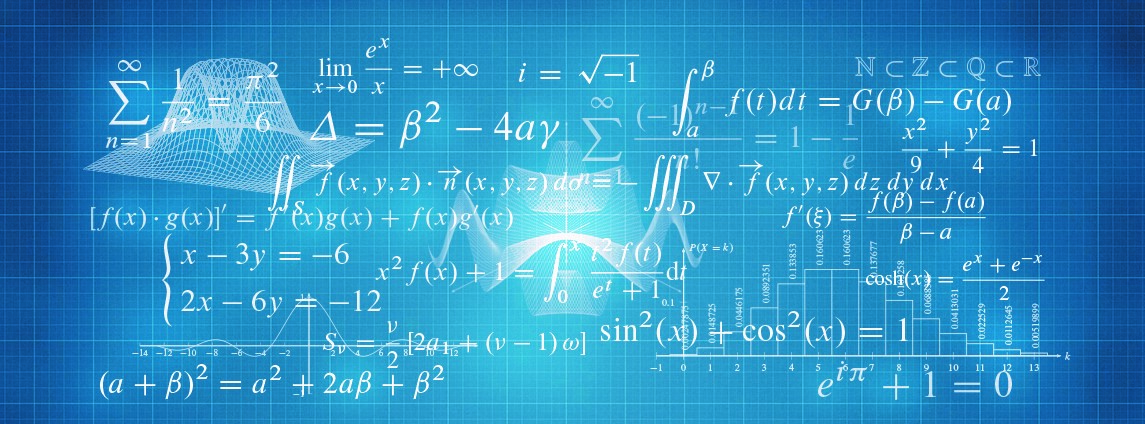
\includegraphics[width=17cm]{Kefalaio}};
\node[anchor=west,xshift=.1\paperwidth,yshift=.14\paperheight,rectangle]
{{\color{white}\fontsize{30}{20}\textbf{\textcolor{black}{\contour{white}{ΚΕΦΑΛΑΙΟ}}}}};
\node[anchor=west,xshift=.09\paperwidth,yshift=.08\paperheight,rectangle] {\fontsize{24}{20} {\color{black}{{\textcolor{black}{\contour{white}{\sc##1}}}}}};
%\fill[fill=black] (12.2,2) rectangle (14.8,4.7);
\node[anchor=west,xshift=.74\paperwidth,yshift=.11\paperheight,rectangle]
{{\color{white}\fontsize{80}{20}\textbf{\textit{\textcolor{white}{\contour{black}{\thechapter}}}}}};
\end{tikzpicture}
};
\end{tikzpicture}
}
\titlespacing*{\chapter}{0pt}{20pt}{30pt}
}
%------------------------------------------------


\usepackage[outline]{contour}
\newcommand{\regularchapter}{%
\titleformat{\chapter}[display]
{\normalfont\huge\bfseries}{\chaptertitlename\ \thechapter}{20pt}{\Huge##1}
\titlespacing*{\chapter}
{0pt}{-20pt}{40pt}
}

\apptocmd{\mainmatter}{\fancychapter}{}{}
\apptocmd{\backmatter}{\regularchapter}{}{}
\apptocmd{\frontmatter}{\regularchapter}{}{}

\titlespacing*{\section}
{0pt}{30pt}{0pt}
\usepackage{booktabs}
\usepackage{hhline}
\DeclareRobustCommand{\perthousand}{%
\ifmmode
\text{\textperthousand}%
\else
\textperthousand
\fi}


\contentsmargin{0cm}
\titlecontents{part}[-1pc]
{\addvspace{10pt}%
\bf\Large ΜΕΡΟΣ\quad }%
{}
{}
{\;\dotfill}%
%------------------------------------------
\titlecontents{chapter}[0pc]
{\addvspace{30pt}%
\begin{tikzpicture}[remember picture, overlay]%
\draw[fill=black,draw=black] (-.3,.5) rectangle (3.7,1.1); %
\pgftext[left,x=0cm,y=0.75cm]{\color{white}\sc\Large\bfseries Κεφάλαιο\ \thecontentslabel};%
\end{tikzpicture}\large\sc}%
{}
{}
{\hspace*{-2.3em}\hfill\normalsize Σελίδα \thecontentspage}%
\titlecontents{section}[2.4pc]
{\addvspace{1pt}}
{\contentslabel[\thecontentslabel]{2pc}}
{}
{\;\dotfill\;\small \thecontentspage}
[]
\titlecontents*{subsection}[4pc]
{\addvspace{-1pt}\small}
{}
{}
{\ --- \small\thecontentspage}
[ \textbullet\ ][]

\makeatletter
\renewcommand{\tableofcontents}{%
\chapter*{%
\vspace*{-20\p@}%
\begin{tikzpicture}[remember picture, overlay]%
\pgftext[right,x=12cm,y=0.2cm]{\Huge\sc\bfseries \contentsname};%
\draw[fill=black,draw=black] (9.5,-.75) rectangle (12.5,1);%
\clip (9.5,-.75) rectangle (15,1);
\pgftext[right,x=12cm,y=0.2cm]{\color{white}\Huge\bfseries \contentsname};%
\end{tikzpicture}}%
\@starttoc{toc}}
\makeatother

\usepackage[contents={},scale=1,opacity=1,color=black,angle=0]{background}

\newcommand\blfootnote[1]{%
\begingroup
\renewcommand\thefootnote{}\footnote{#1}%
\addtocounter{footnote}{-1}%
\endgroup
}
\usepackage{epstopdf}
\epstopdfsetup{update}
\usepackage{textcomp}

\titleformat{\section}
{\normalfont\Large\bf}%
{}{0em}%
{{\color{black}\titlerule[0pt]}\vskip-.2\baselineskip{\parbox[t]{\dimexpr\textwidth-2\fboxsep\relax}{\raggedright\strut\itshape{\LARGE{\thesection~#1}}\strut}}}[\vskip 0\baselineskip{\color{black}\titlerule[1pt]}]
\titlespacing*{\section}{0pt}{0pt}{30pt}

\newcommand{\methodologia}{\begin{center}
{\large \textbf{ΜΕΘΟΔΟΛΟΓΙΑ}}\\\vspace{-2mm}
\begin{tikzpicture}
\shade[left color=white, right color=black,] (-3cm,0) rectangle (0,.2mm);
\shade[left color=black, right color=white,] (0,0) rectangle (3cm,.2mm);   
\end{tikzpicture}
\end{center}}

\newcommand{\orismoi}{\begin{center}
\vspace{-3mm}{\large \textbf{\textcolor{\xrwma}{ΟΡΙΣΜΟΙ}}}\\\vspace{-2mm}
\begin{tikzpicture}
\shade[left color=white, right color=cyan!80!black,] (-3cm,0) rectangle (0,.2mm);
\shade[left color=cyan!80!black, right color=white,] (0,0) rectangle (3cm,.2mm);   
\end{tikzpicture}
\end{center}}
\newcommand{\thewrhmata}{\begin{center}
{\large \textbf{\textcolor{\xrwmath}{ΘΕΩΡΗΜΑΤΑ - ΠΟΡΙΣΜΑΤΑ - ΠΡΟΤΑΣΕΙΣ\\ΚΡΙΤΗΡΙΑ - ΙΔΙΟΤΗΤΕΣ}}}\\\vspace{-2mm}
\begin{tikzpicture}
\shade[left color=white, right color=\xrwmath,] (-5cm,0) rectangle (0,.2mm);
\shade[left color=\xrwmath, right color=white,] (0,0) rectangle (5cm,.2mm);   
\end{tikzpicture}
\end{center}}
\usepackage[labelfont={footnotesize,it,bf},font={footnotesize}]{caption}

%-------- ΠΙΝΑΚΕΣ ---------
\usepackage{booktabs}
%----------------------
%----- ΥΠΟΛΟΓΙΣΤΗΣ ----------
%\usepackage{calculator}
%----------------------------

%----- ΟΡΙΖΟΝΤΙΑ ΛΙΣΤΑ ------
\usepackage{xparse}
\newcounter{answers}
\renewcommand\theanswers{\arabic{answers}}
\ExplSyntaxOn
\NewDocumentCommand{\results}{m}
{
\seq_set_split:Nnn \l_results_a_seq {,}{#1}
\par\nobreak\noindent\setcounter{answers}{0}
\seq_map_inline:Nn \l_results_a_seq
{
\makebox[.18\linewidth][l]{\stepcounter{answers}\theanswers.~##1}\hfill
}
\par
}
\seq_new:N \l_results_a_seq
\ExplSyntaxOff
%----------------------------
%------ ΜΗΚΟΣ ΓΡΑΜΜΗΣ ΚΛΑΣΜΑΤΟΣ ---------
\DeclareRobustCommand{\frac}[3][0pt]{%
{\begingroup\hspace{#1}#2\hspace{#1}\endgroup\over\hspace{#1}#3\hspace{#1}}}
%----------------------------------------
\usepackage{microtype}
\usepackage{float}

\usepackage{caption}

%---- ΟΡΙΖΟΝΤΙΟ - ΚΑΤΑΚΟΡΥΦΟ - ΠΛΑΓΙΟ ΑΓΚΙΣΤΡΟ ------
\newcommand{\orag}[3]{\node at (#1)
{$ \overcbrace{\rule{#2mm}{0mm}}^{{\scriptsize #3}} $};}

\newcommand{\kag}[3]{\node at (#1)
{$ \undercbrace{\rule{#2mm}{0mm}}_{{\scriptsize #3}} $};}

\newcommand{\Pag}[4]{\node[rotate=#1] at (#2)
{$ \overcbrace{\rule{#3mm}{0mm}}^{{\rotatebox{-#1}{\scriptsize$#4$}}}$};}
%-----------------------------------------
\tikzstyle{pl}=[line width=0.3mm]
\tikzstyle{plm}=[line width=0.4mm]
%------- ΣΤΥΛ ΠΑΡΑΔΕΙΓΜΑΤΟΣ -------
\newcounter{paradeigma}[section]
\renewcommand{\theparadeigma}{\bf\thechapter.\arabic{paradeigma}}   
\newcommand{\Paradeigma}[1]{\refstepcounter{paradeigma}\textcolor{cyan}{\textbf{{\large Παράδειγμα\hspace{2mm}\theparadeigma\;:\;}\hspace{1mm}}} \MakeUppercase{\textbf{#1}}\\}{}
%-----------------------------------

%------- ΣΤΥΛ ΛΥΣΗΣ ------------------
\newcommand{\lysh}{{\textbf{ΛΥΣΗ}}}
%------------------------------------

%------ ΛΥΜΕΝΑ ΠΑΡΑΔΕΙΓΜΑΤΑ ΤΙΤΛΟΣ ---------
\newcommand{\Lymena}{\begin{center}
\begin{tikzpicture}
\path[left color=cyan!70!black,right color=cyan!80!black,middle color=cyan!80!white] (-7cm,-.6cm) rectangle (6.5cm,.6cm);
\node at (-.25cm,0) {\Large \textcolor{white}{\textbf{ΛΥΜΕΝΑ ΠΑΡΑΔΕΙΓΜΑΤΑ}}};  
\end{tikzpicture}
\end{center}}
%--------------------------------------

%--------- ΑΛΥΤΕΣ ΑΣΚΗΣΕΙΣ ΤΙΤΛΟΣ ----------
\newcommand{\Alyta}{\begin{center}
\begin{tikzpicture}
\path[left color=cyan!70!black,right color=cyan!80!black,middle color=cyan!80!white] (-7cm,-.6cm) rectangle (6.5cm,.6cm);
\node at (-.25cm,0) {\Large \textcolor{white}{\textbf{ΑΣΚΗΣΕΙΣ - ΠΡΟΒΛΗΜΑΤΑ}}};  
\end{tikzpicture}
\end{center}}
%--------------------------------------------
\usetikzlibrary{shadows,calc}
\usepackage{tcolorbox}
\tcbuselibrary{skins,theorems,breakable}
%---------- ΜΕΘΟΔΟΣ --------------
\newcounter{Methodos}[chapter]
\renewcommand{\theMethodos}{\thechapter.\arabic{Methodos}}
\newenvironment{Methodos}[2][\linewidth]
{\refstepcounter{Methodos}
\begin{tcolorbox}[breakable,
enhanced standard,
boxrule=0.7pt,titlerule=-.2pt,drop fuzzy shadow southeast=black!50,
width=\linewidth,
title style={color=white},
overlay unbroken and first={
\path[left color=cyan!70!black,right color=cyan,draw=black]
([yshift=-\pgflinewidth]frame.north west) to ([yshift=-5pt]title.south west)[rounded corners=2pt] -- ([xshift=-#2-15pt,yshift=-5pt]title.south east) to[rounded corners=2pt] ([xshift=-#2,yshift=-\pgflinewidth]frame.north east) -- cycle;
},
fonttitle=\bfseries,
before=\par\medskip\noindent,
after=\par\medskip,
toptitle=3pt,
top=11pt,topsep at break=-5pt,
colback=white,title={\large Μέθοδος \theMethodos} : {\textcolor{black}{\MakeUppercase{#1}}}]}
{\end{tcolorbox}}
%------------------------------------------
%---------- ΛΙΣΤΕΣ ----------------------
\newlist{bhma}{enumerate}{3}
\setlist[bhma]{label=\bf\textit{\arabic*\textsuperscript{o}\;Βήμα :},leftmargin=0cm,itemindent=1.5cm,ref=\bf{\arabic*\textsuperscript{o}\;Βήμα}}
\newlist{rlist}{enumerate}{3}
\setlist[rlist]{itemsep=0mm,label=\roman*.}
\newlist{alist}{enumerate}{3}
\setlist[alist]{itemsep=0mm,label=\alph*.}
\makeatletter
\renewrobustcmd{\anw@true}{\let\ifanw@\iffalse}
\renewrobustcmd{\anw@false}{\let\ifanw@\iffalse}\anw@false
\newrobustcmd{\noanw@true}{\let\ifnoanw@\iffalse}
\newrobustcmd{\noanw@false}{\let\ifnoanw@\iffalse}\noanw@false
\renewrobustcmd{\anw@print}{\ifanw@\ifnoanw@\else\numer@lsign\fi\fi}
\makeatother

%----ΣΤΥΛ ΑΣΚΗΣΗΣ ----------
\newcounter{askhsh}[chapter]
\renewcommand{\theaskhsh}{\bf{\textit{{\large{\thechapter}}.\arabic{askhsh}}}}   
\newcommand{\Askhsh}{\refstepcounter{askhsh}\textcolor{\xrwma}{{\theaskhsh}\hspace{1mm}}}{}
%---------------------------

\newlist{brlist}{enumerate}{3}
\setlist[brlist]{itemsep=0mm,label=\bf\roman*.}
\newlist{tropos}{enumerate}{3}
\setlist[tropos]{label=\bf\textit{\arabic*\textsuperscript{oς}\;Τρόπος :},leftmargin=0cm,itemindent=2.3cm,ref=\bf{\arabic*\textsuperscript{oς}\;Τρόπος}}
% Αν μπει το bhma μεσα σε tropo τότε
%\begin{bhma}[leftmargin=.7cm]
\newcommand{\tss}[1]{\textsuperscript{#1}}
\newcommand{\tssL}[1]{\MakeLowercase{\textsuperscript{#1}}}
%------------------------------------------
\setlength{\parindent}{0pt}
\setlist[itemize]{itemsep=0mm}
\tkzSetUpPoint[size=7,fill=white]
\newcommand{\twocolkentro}[1]{
\twocolumn[
\begin{@twocolumnfalse}
#1
\end{@twocolumnfalse}]}
\newcommand{\bcc}[1]{
\begin{center}
{\color{\xrwma}{\rule{1cm}{.4pt}}\raisebox{-2.5mm}{\rule{.4pt}{5mm}}}\hspace{1em}\raisebox{-.65ex}{\begin{varwidth}{\dimexpr0.7\textwidth-2em\relax}\centering{\textbf{\textcolor{\xrwma}{\large\scfont\textsc{#1}}}}\end{varwidth}}\hspace*{1em}{\color{\xrwma}{\raisebox{-2.5mm}{\rule{.4pt}{5mm}}\hrulefill}}
\end{center}}

\DeclareMathSizes{10.95}{10.95}{7}{5}
\DeclareMathSizes{6}{6}{3.8}{2.7}
\DeclareMathSizes{8}{8}{5.1}{3.6}
\DeclareMathSizes{9}{9}{5.8}{4.1}
\DeclareMathSizes{10}{10}{6.4}{4.5}
\DeclareMathSizes{12}{12}{7.7}{5.5}
\DeclareMathSizes{14.4}{14.4}{9.2}{6.5}
\DeclareMathSizes{17.28}{17.28}{11}{7.9}
\DeclareMathSizes{20.74}{20.74}{13.3}{9.4}
\DeclareMathSizes{24.88}{24.88}{16}{11.3}

\makeatletter
\AtBeginDocument{
\check@mathfonts
\fontdimen16\textfont2=2.5pt
\fontdimen17\textfont2=2.5pt
\fontdimen14\textfont2=4.5pt
\fontdimen13\textfont2=4.5pt 
}
\makeatother





\begin{document}
\mainmatter
\pagestyle{fancy}
\chapter{Συστήματα} 
\section{Γραμμικά Συστήματα}
\orismoi
\Orismos{Γραμμική Εξίσωση}
Γραμμική εξίσωση δύο μεταβλητών, ονομάζεται κάθε πολυωνυμική εξίσωση της μορφής \[ ax+\beta y=\gamma \]
\begin{itemize}[itemsep=0mm]
\item Οι μεταβλητές της εξίσωσης είναι οι $ x,y $.
\item Οι πραγματικοί αριθμοί $ a,\beta $ λέγονται \textbf{συντελεστές} των μεταβλητών.
\item Ο πραγματικός αριθμός $ \gamma $ ονομάζεται \textbf{σταθερός όρος} της εξίσωσης.
\end{itemize}
\Orismos{Λύση γραμμικήσ εξίσωσησ}
Λύση μιας γραμμικής εξίσωσης της μορφής \[ ax+\beta y=\gamma \] ονομάζεται κάθε διατεταγμένο ζεύγος αριθμών $ \left( x_0,y_0\right)  $ το οποίο επαληθεύει την εξίσωση.\\\\
\Orismos{Γραμμικό σύστημα $ \mathbold{2\times2} $}
Γραμμικό σύστημα δύο εξισώσεων με δύο άγνωστους ονομάζεται ο συνδυασμός - σύζευξη δύο γραμμικών εξισώσεων. Είναι της μορφής :
\begin{equation}\label{systhma}
\ccases{{a}x+{\beta} y={\gamma}\\{a'}x+{\beta'} y={\gamma'} }
\end{equation}
\begin{itemize}[itemsep=0mm]
\item Οι αριθμοί $ a,a',\beta,\beta'\in\mathbb{R} $ ονομάζονται \textbf{συντελεστές} του συστήματος ενώ οι $ \gamma,\gamma'\in\mathbb{R} $ λέγονται \textbf{σταθεροί όροι}.
\item Κάθε διατεταγμένο ζεύγος αριθμών $ \left(x_0,y_0\right)  $ το οποίο επαληθεύει και τις δύο εξισώσεις ονομάζεται \textbf{λύση} του γραμμικού συστήματος.
\item Τα συστήματα τα οποία έχουν ακριβώς τις ίδιες λύσεις ονομάζονται \textbf{ισοδύναμα}.
\item Ένα σύστημα που έχει λύση λέγεται \textbf{συμβιβαστό}. Εάν δεν έχει λύση ονομάζεται \textbf{αδύνατο} ενώ αν έχει άπειρες λύσεις \textbf{αόριστο}.
\end{itemize}
\Orismos{Επαλήθευση Συστήματοσ}
Επαλήθευση ενός συστήματος εξισώσεων ονομάζεται η διαδικασία με την οποία εξετάζουμε εάν ένα ζεύγος αριθμών $ \left(x_0,y_0\right)  $ είναι λύση του, αντικαθιστώντας τους αριθμούς στη θέση των μεταβλητών.\\\\
\Orismos{Ορίζουσα Συστήματοσ {$ \mathbold{2\mathbold{\times}2} $}}
Θεωρούμε ένα γραμμικό σύστημα $ 2\times2 $ της μορφής \eqref{systhma}. Ορίζουσα των συντελεστών ονομάζεται ο αριθμός $ a\beta'-a'\beta $ και συμβολίζεται με $ D $. Μπορεί να γραφτεί στη μορφή πίνακα όπως φαίνεται παρακάτω:
\[ D=\left|\begin{array}{cc}
a & \beta \\ 
a' & \beta'
\end{array}  \right|  \]
Επίσης $ D_x,D_y $ είναι οι ορίζουσες των μεταβλητών που προκύπτουν αν αντικαταστήσουμε στην ορίζουσα $ D $ τη στήλη των συντελεστών των μεταβλητών $ x,y $ αντίστοιχα με τους σταθερούς όρους $ \gamma,\gamma' $. Θα είναι:
\[ D_x=\left|\begin{array}{cc}
\gamma & \beta \\ 
\gamma' & \beta'
\end{array}  \right|\quad,\quad D_y=\left|\begin{array}{cc}
a & \gamma \\ 
a' & \gamma'
\end{array}  \right| \]
\Orismos{Γραμμικό Σύστημα Εξισώσεων $ \mathbold{3\times3} $}
Γραμμικό σύστημα τριών εξισώσεων με τρεις άγνωστους ονομάζεται ένας συνδυασμός από τρεις γραμμικές εξισώσεις της μορφής
\[ \ccases{{a_1}x+{\beta_1} y+{\gamma_1} z=\delta_1\\{a_2}x+{\beta_2} y+{\gamma_2} z=\delta_2\\{a_3}x+{\beta_3} y+{\gamma_3} z=\delta_3} \]
με $ a_i,\beta_i,\gamma_i,\delta_i\in\mathbb{R}\;,\;i=1,2,3 $. Κάθε διατεταγμένη τριάδα αριθμών $ \left( x_0,y_0,z_0\right)  $ η οποία επαληθεύει και τις τρεις εξισώσεις ονομάζεται \textbf{λύση} του γραμμικού συστήματος $ 3\times3 $.\\\\
\Orismos{Παραμετρικό σύστημα}
Παραμετρικό ονομάζεται το γραμμικό σύστημα του οποίου οι συντελεστές ή και οι σταθεροί όροι δίνονται με τη βοήθεια μιας ή περισσότερων παραμέτρων. Η διαδικασία επίλυσης ενός παραμετρικού συστήματος ονομάζεται \textbf{διερεύνηση}.
\\\\
\thewrhmata
\Thewrhma{Γραφική παράσταση εξίσωσης}
Δίνεται η γραμμική εξίσωση με δύο μεταβλητές της μορφής $ ax+\beta y=\gamma $. Για τις διάφορες τιμές των συντελεστών $ a,\beta $ καθώς και του σταθερού όρου $ \gamma $ θα μελετήσουμε τη γραφική αναπαράσταση της εξίσωσης.\\
\wrapr{-4mm}{10}{4.5cm}{4mm}{
\begin{tikzpicture}[domain=-.2:4,y=1cm,scale=.8]
\draw[-latex] (-.5,0) -- coordinate (x axis mid) (4.4,0) node[right,fill=white] {{\footnotesize $ x $}};
\draw[-latex] (0,-.5) -- (0,3.5) node[above,fill=white] {{\footnotesize $ y $}};
\draw[domain=-.2:3.4,samples=100,line width=.4mm,\xrwma] plot function{-0.8*x+2.5};
\tkzText(2.5,2.7){$ ax+\beta y=\gamma $}
\tkzText(2.5,2.2){{\footnotesize $ a,\beta,\gamma\in\mathbb{R} $}}
\tkzText(2.5,1.7){{\footnotesize $ a\neq0 $ ή $ \beta\neq0 $}}
\tkzDefPoint(0,0){O}
\tkzLabelPoint[below left](O){$ O $}
\end{tikzpicture}}{
\begin{rlist}
\item Αν $ a\neq0 $ ή $ \beta\neq0 $ τότε η εξίσωση παριστάνει πλάγια ευθεία με συντελεστή διεύθυνσης $ \lambda=-\frac{a}{\beta} $.
\item Aν $ a=0 $ και $ \beta\neq0 $ τότε παίρνει τη μορφή $ y=\lambda $ και παριστάνει οριζόντια ευθεία με συντελεστή διεύθυνσης $ \lambda=0 $.
\item Αν $ a\neq0 $ και $ \beta=0 $ τότε η εξίσωση γράφεται στη μορφή $ x=\lambda $ και παριστάνει κατακόρυφη ευθεία. Οι ευθείες αυτές δεν έχουν συντελεστή διεύθυνσης.
\item Τέλος αν $ a=0 $ και $ \beta=0 $ τότε διακρίνουμε τις εξής περιπτώσεις:
\begin{alist}
\item  Αν $ \gamma=0 $ τότε η εξίσωση γίνεται $ 0x+0y=0 $, είναι αόριστη και αντιστοιχεί σε όλο το καρτεσιανό επίπεδο.
\item Αν $ \gamma\neq0 $ τότε η εξίσωση είναι $ 0x+0y=\gamma $, είναι αδύνατη και δεν αντιστοιχεί σε κανένα σημείο.
\end{alist}
\end{rlist}}
\Thewrhma{Σημείο σε ευθεία}
Ένα σημείο $ A(x_0,y_0) $ ανήκει σε μια ευθεία με εξίσωση $ ax+\beta y=\gamma $ αν και μόνο αν οι συντεταγμένες του επαληθεύουν την εξίσωση της.\\\\
\Thewrhma{Λύση συστήματοσ {$ \mathbold{2\mathbold{\times}2} $} με χρήση οριζουσων}
Έστω το γραμμικό σύστημα 
\[ \ccases{{a}x+{\beta} y={\gamma}\\{a'}x+{\beta'} y={\gamma'} } \]
με πραγματικούς συντελεστές και ορίζουσα συντελεστών $ D $.
\begin{rlist}
\item Αν η ορίζουσα των συντελεστών του συστήματος είναι διάφορη του μηδενός δηλαδή $ D\neq0 $ τότε το σύστημα έχει μοναδική λύση. Οι τιμές των μεταβλητών δίνονται από τις σχέσεις
\[ x=\frac{D_x}{D}\;\;,\;\;y=\frac{D_y}{D} \]
ενώ η λύση του συστήματος θα είναι $ (x,y)=\left(\frac{D_x}{D},\frac{D_y}{D} \right)  $.
\item Αν η ορίζουσα των συντελεστών του συστήματος είναι μηδενική δηλαδή $ D=0 $ τότε το σύστημα είναι είτε αόριστο είτε αδύνατο. Συγκεκριμένα
\begin{alist}
\item αν $ D_x\neq0 $ ή $ D_y\neq0 $ τότε το σύστημα είναι αδύνατο.
\item αν $ D_x=0 $ και $ D_y=0 $ τότε το σύστημα είναι αόριστο.
\end{alist}
\end{rlist}
\newpage
\noindent
\Lymena
\begin{Methodos}[Γραμμική εξίσωση - Ευθεία - Κοινά σημεία ]{1cm}
Δεδομένης μιας γραμμικής εξίσωσης μπορούμε να εξετάσουμε ποια σημεία ανήκουν στην ευθεία που παριστάνει καθώς και τα σημεία τομής της ευθείας αυτής με του άξονες.
\begin{itemize}[leftmargin=3mm]
\item \textbf{Σημεία ευθείας}\\
Για να εξετάσουμε αν κάποιο σημείο $ A(x_0,y_0) $ ανήκει στην ευθεία που ορίζει μια γραμμική εξίσωση, αντικαθιστούμε τις συντεταγμένες του $ A $ στη θέση των μεταβλητών της εξίσωσης και εξετάζουμε αν οι αριθμοί αυτοί την επαληθεύουν. Αν ναι τότε το σημείο ανήκει στην ευθεία.
\item \textbf{Σημεία τομής με τους άξονες}\\
Για να βρούμε τα σημεία τομής μιας ευθείας με τους άξονες τότε θέτουμε όπου $ x=0 $ ή $ y=0 $ στη γραμμική εξίσωση για τους άξονες $ y'y $ και $ x'x $ αντίστοιχα.
\end{itemize}
Αν αναζητούμε κοινά σημεία δύο ευθειών τότε λύνουμε το γραμμικό σύστημα που ορίζουν οι εξισώσεις των ευθειών. Την περίπτωση αυτή την εξετάζουμε στη \textbf{Μέθοδο \ref{meth:grafikh}}.
\end{Methodos}
\Paradeigma{Σημείο ευθείας}
\textbf{Να εξεταστεί αν τα σημεία {\boldmath$ A(2,3) $} και {\boldmath$ B(-1,4) $} ανήκουν στην ευθεία {\boldmath$ 2x+y=7 $}.}\\\\
\lysh\\
Αντικαθιστούμε τς συντεταγμένες του σημείου $ A(2,3) $ στην εξίσωση και έχουμε αναλυτικά :
\[ \textrm{Για }x=2\ \textrm{και }y=3\Rightarrow 2\cdot 2+3=7\Rightarrow 4+3=7\Rightarrow 7=7 \]
Η εξίσωση επαληθεύεται οπότε το σημείο $ A $ ανήκει στην ευθεία. Ομοίως για το σημείο $ B $ θα έχουμε :
\[ \textrm{Για }x=-1\ \textrm{και }y=4\Rightarrow 2\cdot (-1)+4=7\Rightarrow -2+4=7\Rightarrow 2=7 \]
Η εξίσωση δεν επαληθεύεται οπότε το σημείο $ B $ δεν ανήκει στην ευθεία.\\\\
\Paradeigma{Σημεία τομής με τους άξονες}
\textbf{Να βρεθούν τα σημεία τομής της ευθείας {\boldmath$ 3x+4y=6 $} με τους άξονες {\boldmath$ x'x,y'y $}.}\\\\
\lysh\\
Επιλέγουμε $ x=0 $ και $ y=0 $ αντίστοιχα και θα έχουμε :\\
\wrapr{-11mm}{7}{3.5cm}{-11mm}{\begin{tikzpicture}

\begin{axis}[belh ar,aks_on,xmin=-.2,xmax=3,ymin=-.2,
ymax=2.5,xlabel={\footnotesize$x$},ylabel={\footnotesize$y$},x=1cm,y=1cm]
\addplot[domain=-.3:2.5,grafikh parastash]{-3*x/4+3/2};
\coordinate (B) at (axis cs:2,0);
\coordinate (A) at (axis cs:0,1.5);
\end{axis}
\tkzDrawPoints(A,B)
\tkzLabelPoint[above right](A){\footnotesize$A\left(0,\frac{3}{2}\right)$}
\tkzLabelPoint[above right](B){\footnotesize$B(2,0)$}
\end{tikzpicture}}{
\begin{itemize}[leftmargin=4mm]
\item Για το σημείο του άξονα $ y'y $ έχουμε $ x=0 $ άρα $ 3\cdot0+4y=6\Rightarrow y=\frac{3}{2} $. Το σημείο θα είναι $ A\left( 0,\frac{3}{2}\right)  $.
\item Για το σημείο του άξονα $ x'x $ έχουμε $ y=0 $ άρα $ 3x+4\cdot0=6\Rightarrow x=2 $. Το σημείο θα είναι $ B(2,0) $.
\end{itemize}}
\begin{Methodos}[Μέθοδος της αντικατάστασης]{3cm}
Για την επίλυση ενός συστήματος με δύο μεταβλητές έστω $ x,y $ με τη μέθοδο της αντικατάστασης ακολουθούμε τα παρακάτω βήματα.
\begin{bhma}
\item \textbf{Επιλογή εξίσωσης}\\
Επιλέγουμε μια απ' τις δύο εξισώσεις ώστε να λύσουμε ως προς οποιαδήποτε μεταβλητή. Θα προκύψει μια σχέση (1) που θα μας δίνει την μεταβλητή αυτή ως συνάρτηση της άλλης. 
\item \textbf{Αντικατάσταση}\\
Τη μεταβλητή αυτή την αντικαθιστούμε στην άλλη εξίσωση του συστήματος οπότε προκύπτει μια εξίσωση με έναν άγνωστο. Λύνοντας την εξίσωση υπολογίζουμε τον άγνωστο αυτό.
\item \textbf{Υπολογισμός 2\tss{ου} αγνώστου}\\
Την τιμή που θα βρούμε για τη μια μεταβλητή λύνοντας την εξίσωση, την αντικαθιστούμε στη σχέση (1) ώστε να βρεθεί και η άλλη μεταβλητή του συστήματος.
\item \textbf{Λύση συστήματος}\\
Όταν βρεθούν οι τιμές $ x_0,y_0 $ και των δύο αγνώστων, σχηματίζουμε το διατεταγμένο ζεύγος $ (x,y)=(x_0,y_0) $ το οποίο είναι η λύση του συστήματος.
\end{bhma}
\end{Methodos}
\Paradeigma{Λύση συστήματος με αντικατάσταση}
\textbf{Να λυθεί το παρακάτω σύστημα με τη μέθοδο της αντικατάστασης}
{\boldmath\[ \systeme{2x+3y=5,x-4y=-3} \]}
\lysh\\
Παρατηρούμε οτι η 2\tss{η} εξίσωση είναι εύκολο να λυθεί ως προς $ x $ οπότε έχουμε
\begin{equation}
\systeme{2x+3y=5,x-4y=-3}\Rightarrow x=4y-3
\end{equation}
Αντικαθιστώντας το αποτέλεσμα της σχέσης (1) στην 1\tss{η} εξίσωση προκύπτει :
\begin{equation}\begin{aligned}
2x+3y=5\Rightarrow 2(4y-3)+3y=5&\Rightarrow 8y-6+3y=5\\&\Rightarrow 8y+3y=5+6\Rightarrow 11y=11\Rightarrow y=1\end{aligned}
\end{equation}
Τη λύση της εξίσωσης (2) την αντικαθιστούμε στην (1) για να υπολογίσουμε τον άγνωστο $ x $
\[ x=4y-3=4\cdot1-3=4-3=1 \]
Επομένως η λύση του συστήματος θα είναι η $ (x,y)=(1,1) $.
\begin{Methodos}[Μέθοδος των αντίθετων συντελεστών]{2cm}
Για την επίλυση ενός συστήματος με τη μέθοδο των αντίθετων συντελεστών
\begin{bhma}
\item \textbf{Επιλογή μεταβλητής}\\
Επιλέγουμε ποια από τις δύο μεταβλητές θα απαλείψουμε χρησιμοποιώντας τη μέθοδο αυτή.
\item \textbf{Πολλαπλασιασμός εξισώσεων}\\
Τοποθετούμε δίπλα από κάθε εξίσωση τους συντελεστές την μεταβλητής που επιλέξαμε \textquotedblleft χιαστί\textquotedblright\; αλλάζοντας το πρόσημο του ενός από τους δύο. Πολλαπλασιάζουμε την κάθε εξίσωση με τον αριθμό που προκύπτει.
\item \textbf{Πρόσθεση κατά μέλη}\\
Προσθέτουμε κατά μέλη τις νέες εξισώσεις οπότε προκύπτει μια εξίσωση με έναν άγνωστο τον οποίο και υπολογίζουμε λύνοντας την.
\item \textbf{Εύρεση 2\tss{ης} μεταβλητής}\\
Αντικαθιστούμε το αποτέλεσμα σε οποιαδήποτε εξίσωση του αρχικού συστήματος ώστε να υπολογίσουμε και τη δεύτερη μεταβλητή.
\item \textbf{Λύση συστήματος}\\
Όταν βρεθούν οι τιμές $ x_0,y_0 $ και των δύο αγνώστων, σχηματίζουμε το διατεταγμένο ζεύγος $ (x,y)=(x_0,y_0) $ το οποίο είναι η λύση του συστήματος.
\end{bhma}
\end{Methodos}
\Paradeigma{Λύση συστήματοσ με αντίθετουσ συντελεστέσ}
\textbf{Να λυθεί το παρακάτω σύστημα με τη μέθοδο των αντίθετων συντελεστών}
{\boldmath\[ \systeme{4x-y=5,3x+2y=12} \]}
\lysh\\
Επιλέγουμε με τη μέθοδο αυτή να απαλείψουμε τη μεταβλητή $ y $ του συστήματος. Έχουμε λοιπόν
\[ \left. \systeme{4x-y=5,3x+2y=12}\right| \synt{2}{1}\Rightarrow\systeme{8x-2y=10,3x+2y=12} \]
Οπότε προσθέτοντας τις εξισώσεις κατά μέλη προκύπτει
\begin{center}
\vspace{-5mm}
\begin{equation}\label{par:as}
\begin{tabular}{rr}
$ \displaystyle\systeme{8x-2y=10,3x+2y=12} $  &  \\ 
\hhline{-~} $ 11x=22 $ & $ \Rightarrow x=2  $
\end{tabular}
\end{equation}
\end{center}
Την τιμή αυτή της μεταβλητής $ x $ από τη σχέση \eqref{par:as} την αντικαθιστούμε σε οποιαδήποτε εξίσωση και υπολογίζουμε τη δεύτερη μεταβλητή $ y $.
\begin{equation}\begin{aligned}
3x+2y=12\Rightarrow 3\cdot2+2y=12&\Rightarrow 6+2y=12\\&\Rightarrow 2y=12-6\Rightarrow 2y=6\Rightarrow y=3\end{aligned}
\end{equation}
Από τις σχέσεις (3) και (4) παίρνουμε τη λύση του συστήματος η οποία είναι $ (x,y)=(2,3) $.
\begin{Methodos}[Μέθοδος των οριζουσών]{4cm}
Ένα γραμμικό σύστημα δύο εξισώσεων με δύο άγνωστους μπορούμε πλέον να το λύσουμε με τη χρήση οριζουσών ως εξής.
\begin{bhma}
\item \textbf{Υπολογισμός οριζουσών}\\
Υπολογίζουμε την ορίζουσα $ D $ των συντελεστών του συστήματος καθώς και τις ορίζουσες των μεταβλητών $ D_x $ και $ D_y $.
\item \textbf{Διερεύνηση - Εύρεση λύσεων}\\
Διακρίνουμε τις εξής περιπτώσεις
\begin{itemize}
\item Αν $ D\neq0 $ τότε υπολογίζουμε τις τιμές των μεταβλητών σύμφωνα με το \textbf{Θεώρημα 3} οπότε η μοναδική λύση θα είναι $ (x,y)=\left(\frac{D_x}{D},\frac{D_y}{D} \right) $.
\item Αν $ D=0 $ τότε διακρίνουμε τις εξής περιπτώσεις:
\begin{itemize}
\item Αν $ D_x\neq 0 $ ή $ D_y\neq 0 $ τότε το σύστημα είναι αδύνατο.
\item Αν $ D_x=D_y=0 $ τότε το σύστημα είναι αόριστο.
\end{itemize}
\end{itemize}
\end{bhma}
\end{Methodos}\mbox{}\\\\
\Paradeigma{Λύση συστήματοσ με τη μέθοδο οριζουσών}
\textbf{Να λυθεί το παρακάτω σύστημα}
{\boldmath\[ \systeme{x-5y=3,4x-3y=-5} \]}
\textbf{με τη μέθοδο των οριζουσών}.\\\\
\lysh\\
Η ορίζουσα των συντελεστών του συστήματος θα είναι
\[ D=\begin{vmatrix}
1&-5\\4&-3
\end{vmatrix}=1\cdot(-3)-4\cdot(-5)=-3+20=17 \]
Η ορίζουσα των συντελεστών είναι μη μηδενική οπότε το σύστημα έχει μοναδική λύση. Οι ορίζουσες των μεταβλητών θα είναι
\begin{gather*}
D_x=\begin{vmatrix}
3&-5\\-5&-3
\end{vmatrix}=3\cdot(-3)-(-5)\cdot(-5)=-34\;\textrm{ και }\\D_y=\begin{vmatrix}
1 & 3\\4&-5
\end{vmatrix}=1\cdot(-5)-4\cdot3=-17 \end{gather*}
Σύμφωνα με τα παραπάνω οι τιμές των μεταβλητών του συστήματος θα είναι 
\[ x=\frac{D_x}{D}=\frac{-34}{17}=-2\;\textrm{ και }\;y=\frac{D_y}{D}=\frac{-17}{17}=-1 \]
οι οποίες μας δίνουν τη λύση του συστήματος $ (x,y)=(-2,-1) $.\\\\
\Paradeigma{Λύση συστήματοσ με τη μέθοδο οριζουσών}
\textbf{Να λυθεί το παρακάτω σύστημα με τη μέθοδο των οριζουσών}
{\boldmath\[ \systeme{4x-8y=1,6x-12y=4} \]}
\lysh\\
Υπολογίζουμε την ορίζουσα των συντελεστών
\[ D=\begin{vmatrix}
4& -8\\6 & -12
\end{vmatrix}=4\cdot(-12)-6\cdot(-8)=-48+48=0 \]
Η μηδενική ορίζουσα μας δείχνει ότι το σύστημα είναι είτε αόριστο είτε αδύνατο. Για να προσδιορίσουμε το είδος του υπολογίζουμε τις ορίζουσες $ D_x,D_y $.
\begin{align*}
D_x&=\begin{vmatrix}
1& -8\\4 & -12
\end{vmatrix}=1\cdot(-12)-4\cdot(-8)=-12+32=20\neq 0\\
D_y&=\begin{vmatrix}
4& 1\\6 & 4
\end{vmatrix}=4\cdot 4-1\cdot 6=16-6=10\neq 0
\end{align*}
Οι ορίζουσες των μεταβλητών είναι μη μηδενικές οπότε το σύστημα είναι αδύνατο.\\\\
\Paradeigma{Λύση συστήματοσ με τη μέθοδο οριζουσών}
\textbf{Να λυθεί το παρακάτω σύστημα με τη μέθοδο των οριζουσών}
{\boldmath\[ \systeme{3x-y=5,6x-2y=10} \]}
\lysh\\
Η ορίζουσα του συστήματος θα είναι
\[ D=\begin{vmatrix}
3& -1\\6 & -2
\end{vmatrix}=3\cdot(-2)-6\cdot(-1)=-6+6=0 \]
Θα πρέπει κι εδώ να προσδιορίσουμε αν το σύστημα είναι αδύνατο ή αόριστο. Για να προσδιορίσουμε το είδος του υπολογίζουμε τις ορίζουσες $ D_x,D_y $.
\begin{align*}
D_x&=\begin{vmatrix}
5& -1\\10 & -2
\end{vmatrix}=5\cdot(-2)-(-1)\cdot 10=-10+10=0\\
D_y&=\begin{vmatrix}
3& 5\\6 & 10
\end{vmatrix}=3\cdot 10-5\cdot 6=30-30=0
\end{align*}
Οι ορίζουσες των μεταβλητών είναι μηδενικές οπότε το σύστημα είναι αόριστο. Για να βρούμε τη μορφή όλων των λύσεων τις εκφράζουμε με τη βοήθεια μιας παραμέτρου ως εξής : 
Λύνουμε την πρώτη εξίσωση ως προς $ y $ : 
\begin{equation}\label{par:oraor}
3x-y=5\Rightarrow -y=5-3x\Rightarrow y=3x-5 
\end{equation}
Θέτουμε στη δεύτερη μεταβλητή $ x=\lambda $ και παίρνουμε από τη σχέση \eqref{par:oraor} $ y=3\lambda-5 $. Επομένως οι άπειρες λύσεις δίνονται παραμετρικά από τη σχέση \[ (x,y)=(\lambda,3\lambda-5) \]
\begin{Methodos}[Γραφική επίλυση συστήματο2]{3cm}\label{meth:grafikh}
Ένα γραμμικό σύστημα μπορεί να λυθεί και γεωμετρικά με τη βοήθεια των ευθειών των εξισώσεων.
\begin{bhma}
\item \textbf{Χάραξη των ευθειών}\\
Σχεδιάζουμε τις δύο ευθείες του συστήματος βρίσκοντας για καθεμιά δύο σημεία της με τη βοήθεια της εξίσωσης της.
\item \textbf{Σχετική θέση ευθειών}\\
Διακρίνουμε τις εξής περιπτώσεις για τη σχετική θέση των δύο ευθειών
\begin{itemize}[itemsep=0mm]
\item Αν οι ευθείες \textbf{τέμνονται} σε ένα σημείο τότε οι συντεταγμένες του κοινού αυτού σημείου είναι η ζητούμενη λύση του συστήματος. Τις συντεταγμένες αυτές τις βρίσκουμε σχεδιάζοντας από το σημείο, κάθετες γραμμές προς τους άξονες $ x'x $ και $ y'y $.
\item Αν οι δύο ευθείες είναι μεταξύ τους παράλληλες τότε \textbf{δεν υπάρχουν κοινά σημεία} μεταξύ τους και κατά συνέπεια το σύστημα δεν έχει λύση οπότε είναι \textbf{αδύνατο}.
\item Τέλος αν οι ευθείες \textbf{ταυτίζονται} τότε έχουν μεταξύ τους άπειρα κοινά σημεία οπότε το σύστημα έχει άπειρες λύσεις δηλαδή είναι \textbf{αόριστο}.
\end{itemize}
\vspace{-7mm}
\begin{center}
\begin{tabular}{p{4cm}p{4cm}p{4cm}}
\begin{tikzpicture}
\begin{axis}[aks_on,belh ar,ticks=none,xlabel={\footnotesize $x$},
ylabel={\footnotesize $y$},xmin=-.3,xmax=3.5,ymin=-.3,ymax=3.5,x=.8cm,y=.8cm]
\addplot[grafikh parastash,\xrwmath,domain=-.2:3.3]{-x+2.5};
\addplot[grafikh parastash,\xrwmath,domain=-.2:2.7]{.8*x+.7};
\node (A) at (axis cs:1,1.5){};
\end{axis}
\tkzDrawPoint(A)
\tkzLabelPoint[right](A){$A(x_0,y_0)$}
\node at (0,0) {$O$};
\node at (2,3.4) {\footnotesize {Μοναδική λύση}};
\node at (2,1.9) {\footnotesize $\varepsilon_2$};
\node at (.8,2) {\footnotesize $\varepsilon_1$};
\end{tikzpicture}	& \begin{tikzpicture}
\begin{axis}[aks_on,belh ar,ticks=none,xlabel={\footnotesize $x$},
ylabel={\footnotesize $y$},xmin=-.3,xmax=3.5,ymin=-.3,ymax=3.5,x=.8cm,y=.8cm]
\addplot[grafikh parastash,\xrwmath,domain=-.2:2.5]{x+.7};
\addplot[grafikh parastash,\xrwmath,domain=-.2:3.3]{x-1};
\end{axis}
\node at (0,0) {$O$};
\node at (2,3.4) {\footnotesize {Καμία λύση}};
\node at (2,1.5) {\footnotesize $\varepsilon_2$};
\node at (1,2) {\footnotesize $\varepsilon_1$};
\end{tikzpicture} & \begin{tikzpicture}
\begin{axis}[aks_on,belh ar,ticks=none,xlabel={\footnotesize $x$},
ylabel={\footnotesize $y$},xmin=-.3,xmax=3.5,ymin=-.3,ymax=3.5,x=.8cm,y=.8cm]
\addplot[grafikh parastash,\xrwmath,domain=-.2:3.5]{0.7*x+.5};
\addplot[grafikh parastash,\xrwmath,domain=-.2:3.5,dashed]{0.7*x+.45};
\end{axis}
\node at (0,0) {$O$};
\node at (2,3.4) {\footnotesize {Άπειρες λύσεις}};
\node at (2,1.5) {\footnotesize $\varepsilon_2$};
\node at (1,1.5) {\footnotesize $\varepsilon_1$};
\end{tikzpicture} \\ 
\end{tabular} 
\end{center}
\end{bhma}
\end{Methodos}
\Paradeigma{Γραφική επίλυση συστήματοσ}
\textbf{Να λυθούν γραφικά τα παρακάτω συστήματα}
\begin{multicols}{3}
\begin{brlist}
\item {\boldmath$ \systeme{3x-2y=4,x+y=3} $}
\item {\boldmath$ \systeme{2x-y=5,4x-2y=4} $}
\item {\boldmath$ \systeme{x-3y=1,3x-9y=3} $}
\end{brlist}
\end{multicols}
\noindent
Για κάθε μια από τις εξισώσεις των παραπάνω συστημάτων θα βρούμε δύο ζεύγη αριθμών που τις επαληθεύουν τα οποία θα παριστάνουν σημεία στο επίπεδο έτσι ώστε να σχεδιαστούν οι ευθείες.
\begin{rlist}
\item Στην πρώτη εξίσωση επιλέγουμε $ x=0 $ οπότε έχουμε
\[ 3x-2y=4\Rightarrow 3\cdot0-2y=4\Rightarrow y=-2 \]
Αποκτάμε έτσι το σημείο $ A(0,-2) $. Ένα δεύτερο σημείο θα βρεθεί παίρνοντας π.χ. $ y=0 $ οπότε με πράξεις προκύπτει
\[ 3x-2y=4\Rightarrow 3χ-2\cdot0=4\Rightarrow3x=4\Rightarrow y=\frac{4}{3} \]
Προκύπτει έτσι το σημείο $ B\left( \frac{4}{3},0\right) $. Με παρόμοιο τρόπο υπολογίζουμε δύο σημεία και της 2\tss{ης} ευθείας. Έχουμε από τη 2\tss{η} εξίσωση για $ y=0 $\\
\wrapr{-7mm}{12}{4.5cm}{-7mm}{\begin{tikzpicture}
\begin{axis}[aks_on,belh ar,xlabel={\footnotesize $x$},
ylabel={\footnotesize $y$},xmin=-.3,xmax=3.5,ymin=-.3,ymax=3.5,x=1cm,y=1cm]
\addplot[grafikh parastash,\xrwmath,domain=-.2:3.3]{1.5*x-2};
\addplot[grafikh parastash,\xrwmath,domain=-.2:3.2]{3-x};
\draw[dashed] (axis cs:2,0)--(axis cs:2,1)--(axis cs:0,1);
\node (A) at (axis cs:2,1){};
\end{axis}
\tkzDrawPoint(A)
\tkzLabelPoint[right](A){$M(2,1)$}
\node at (0,0) {$O$};
\node at (2.4,2) {\footnotesize $\varepsilon_2$};
\node at (1.2,2) {\footnotesize $\varepsilon_1$};
\end{tikzpicture}}{
\[ x+y=3\Rightarrow x+0=3\Rightarrow x=3 \] και παίρνουμε έτσι το σημείο $ \varGamma(3,0) $. Επίσης για $ x=0 $
\[ x+y=3\Rightarrow 0+y=3\Rightarrow y=3 \] άρα το δεύτερο σημείο της θα είναι το $ \varDelta(0,3) $. Σχεδιάζοντας τις δύο ευθείες προκύπτει το διπλανό σχήμα. Από το σχήμα αυτό παρατηρούμε ότι οι δύο ευθείες έχουν ένα κοινό σημείο $ M $. Από το σημείο αυτό αν σχεδιάσουμε κάθετες γραμμές πάνω στους άξονες $ x'x $ και $ y'y $ προκύπτουν οι συντεταγμένες του κοινού σημείου οι οποίες είναι $ (x,y)=(2,1) $. Οι συντεταγμένες αυτές είναι η λύση του συστήματος.\\}
\item Με παρόμοιο τρόπο όπως και στο προηγούμενο παράδειγμα δύο σημεία για κάθε ευθεία είναι τα $ A(1,0) $, $ B(0,1) $ και $ \varGamma(2,-1) $, $ \varDelta(2{,}5,0) $ αντίστοιχα. Σχεδιάζοντας τις δύο ευθείες στο σύστημα συντεταγμένων παρατηρούμε ότι είναι παράλληλες άρα δεν έχουν κοινά σημεία οπότε το σύστημα είναι αδύνατο.
\item Σχεδιάζοντας τις ευθείες και του τρίτου συστήματος με τον τρόπο που είδαμε στα προηγούμενα παραδείγματα παρατηρούμε ότι ταυτίζονται. Αυτό σημαίνει ότι έχουν άπειρα κοινά σημεία και κατά συνέπεια το σύστημα είναι αόριστο.
\begin{center}
\begin{tabular}{cc}
\begin{tikzpicture}
\begin{axis}[aks_on,belh ar,xlabel={\footnotesize $x$},
ylabel={\footnotesize $y$},xmin=-.3,xmax=3.5,ymin=-1,ymax=2.5,x=1cm,y=1cm]
\addplot[grafikh parastash,\xrwmath,domain=-.2:3.3]{2*x-1};
\addplot[grafikh parastash,\xrwmath,domain=-.2:3.2]{2*x-3.5};
\end{axis}
\node at (0,.8) {$O$};
\node at (2.7,3) {\footnotesize $\varepsilon_2$};
\node at (1.1,2.7) {\footnotesize $\varepsilon_1$};
\node at (3,0.4) {\footnotesize {Καμία λύση}};
\end{tikzpicture}	& \begin{tikzpicture}
\begin{axis}[aks_on,belh ar,xlabel={\footnotesize $x$},
ylabel={\footnotesize $y$},xmin=-.3,xmax=3.5,ymin=-1,ymax=2.5,x=1cm,y=1cm]
\addplot[grafikh parastash,\xrwmath,domain=-.2:3.3]{x/3-1/3};
\addplot[grafikh parastash,\xrwmath,domain=-.2:3.2,dashed]{x/3-1/3-.05};
\end{axis}
\node at (0,0.75) {$O$};
\node at (2.7,1.2) {\footnotesize $\varepsilon_2$};
\node at (1.2,1.2) {\footnotesize $\varepsilon_1$};
\node at (2,2.5) {\footnotesize {Άπειρες λύσεις}};
\end{tikzpicture} \\ 
\end{tabular} 
\end{center}
\end{rlist}
\begin{Methodos}[Επίλυση σύνθετου συστήματος]{3cm}
Αν μας ζητείται να λύσουμε ένα σύστημα του οποίου οι εξισώσεις δεν είναι στην απλή γραμμική μορφή όπως φαίνεται στον \textbf{Ορισμό 3}, τότε
\begin{bhma}
\item \textbf{Πράξεις}\\
Εκτελούμε πράξεις και στα δύο μέλη κάθε εξίσωσης και διαχωρίζουμε τους γνωστούς από τους άγνωστους όρους, ώστε να τις φέρουμε σε γραμμική μορφή.
\item \textbf{Λύση γραμμικού συστήματος}\\
Λύνουμε το γραμμικό πλέον σύστημα με οποιαδήποτε μέθοδο μας συμφέρει, επιλέγοντας μια από τις \textbf{Μεθόδους 1,2,3} και \textbf{4}.
\end{bhma}
\end{Methodos}
\Paradeigma{Σύνθετο σύστημα}
\textbf{Να λυθεί το παρακάτω σύστημα με οποιαδήποτε μέθοδο.}
{\boldmath\[ \ccases{
\;\dfrac{x+2}{3}+\dfrac{1-y}{2}=2\\
\;\dfrac{2x-1}{5}+\dfrac{y}{3}=-\dfrac{2}{15}} \]}
\lysh\\
Η μορφή στην οποία βρίσκεται κάθε εξίσωση του συστήματος δεν είναι η απλή γραμμική. Αυτό σημαίνει ότι δεν μπορεί να εφαρμοστεί ακόμα κάποια από τις μεθόδους επίλυσης. Κάνοντας πράξεις θα απλοποιήσουμε τη μορφή του συστήματος.
\begin{gather*}
\ccases{
\;\dfrac{x+2}{3}+\dfrac{1-y}{2}=2\\
\;\dfrac{2x-1}{5}+\dfrac{y}{3}=-\dfrac{2}{15}}\Rightarrow\ccases{
\;6\dfrac{x+2}{3}+6\dfrac{1-y}{2}=2\cdot 6\\[2mm]
\;15\dfrac{2x-1}{5}+15\dfrac{y}{3}=-15\dfrac{2}{15}}\Rightarrow\\
\ccases{
\;2(x+2)+3(1-y)=12\\
\;3(2x-1)+5y=-2}\Rightarrow\ccases{2x+4+3-3y=12\\6x-3+5y=-2}\Rightarrow\ccases{2x-3y=5\\6x+5y=1}
\end{gather*}
Το τελευταίο σύστημα έχει τη ζητούμενη μορφή οπότε μπορούμε να το λύσουμε με μια από τις παραπάνω μεθόδους. Με τη μέθοδο των οριζουσών έχουμε :
\[ D=\begin{vmatrix}
2& -3\\6& 5
\end{vmatrix}=28\;,\;D_x=\begin{vmatrix}
5& -3\\1& 5
\end{vmatrix}=28\;,\;D_y=\begin{vmatrix}
2& 5\\6& 1
\end{vmatrix}=-28 \]
Οπότε οι τιμές των δύο μεταβλητών είναι $ x=\frac{D_x}{D}=\frac{28}{28}=1 $ και $ y=\frac{D_y}{D}=\frac{-28}{28}=-1 $ που μας δίνουν τη λύση $ (x,y)=(1,-1) $.
\begin{Methodos}[Επίλυση συστήματος {$\mathbold{3\times 3}$}]{4cm}
Για να λυθεί ένα $ 3\times 3 $ γραμμικό σύστημα με μεταβλητές έστω $ x,y,z $, θα χρησιμοποιήσουμε τη μέθοδο της αντικατάστασης ώστε να μεταβούμε σε ένα $ 2\times 2 $ γραμμικό σύστημα.
\begin{bhma}
\item \textbf{Επιλογή εξίσωσης}\\
Επιλέγουμε μια από τις τρεις εξισώσεις για να λύσουμε ως προς οποιονδήποτε άγνωστο.
\item \textbf{Αντικατάσταση}\\
Αντικαθιστούμε τη μεταβλητή αυτή στις υπόλοιπες δύο εξισώσεις του συστήματος με αποτέλεσμα να μετατραπούν σε γραμμικές εξισώσεις με δύο άγνωστους.
\item \textbf{Επίλυση συστήματος {\boldmath{$ 2\times 2 $}}}\\
Απλοποιούμε τις δύο νέες εξισώσεις ώστε να τις φέρουμε στην απλή γραμμική μορφή και λύνουμε το $ 2\times 2 $ σύστημα με οποιαδήποτε μέθοδο.
\item \textbf{Εύρεση τρίτου αγνώστου}\\
Όταν βρεθούν οι τιμές των δύο μεταβλητών του $ 2\times 2 $ συστήματος τις αντικαθιστούμε στη σχέση που προέκυψε στο \textbf{1\tss{ο} Βήμα} και υπολογίζουμε και τον τρίτο άγνωστο.
\item \textbf{Λύση συστήματος}\\
Σχηματίζουμε τη λύση του αρχικού συστήματος η οποία θα είναι μια διατεταγμένη τριάδα αριθμών της μορφής $ (x,y,z)=(x_0,y_0,z_0) $.
\end{bhma}
\end{Methodos}\mbox{}\\
\Paradeigma{Λύση γραμμικού συστήματοσ {$\mathbold{3\times 3}$}}
\textbf{Να λυθεί το παρακάτω γραμμικό σύστημα}
{\boldmath\[ \systeme{2x-y+3z=8,3x+4y-z=1,x+y-4z=-3} \]}
\lysh\\
Επιλέγουμε την 3\tss{η} εξίσωση προκειμένου να λύσουμε ως προς τη μεταβλητή $ x $ οπότε θα έχουμε
\begin{equation} \systeme{2x-y+3z=8,3x+4y-z=1,x+y-4z=-3}\Rightarrow x=4z-y-3 
\end{equation}
Αντικαθιστώντας τη μεταβλητή $ x $ από τη σχέση (8) στις δύο πρώτες εξισώσεις του συστήματος προκύπτει
\[ \ccases{2(4z-y-3)-y+3z=8\\3(4z-y-3)+4y-z=1}\Rightarrow\ccases{8z-2y-6-y+3z=8\\12z-3y-9+4y-z=1}\Rightarrow
\systeme{-3y+11z=14,y+11z=10} \]
Η μορφή του συστήματος μας επιτρέπει να χρησιμοποιήσουμε ένα τέχνασμα για να φτάσουμε γρήγορα στη λύση. Αφαιρώντας κατά μέλη έχουμε
\begin{equation}
\begin{tabular}{rr}
$  \displaystyle\systeme{-3y+11z=14,y+11z=10} $  &  \\ 
\hhline{-~}  $ -4y=4 $ & $ \Rightarrow y=-1 $
\end{tabular}
\end{equation}
Από την πρώτη εξίσωση και τη σχέση (9) υπολογίζουμε τον άγνωστο $ z $
\begin{equation} -3y+11z=14\Rightarrow-3\cdot(-1)+11z=14\Rightarrow3+11z=14\Rightarrow11z=11\Rightarrow z=1 \end{equation}
Τις τιμές των μεταβλητών $ y,z $ από τις σχέσεις (9) και (10) τις αντικαθιστούμε στην ισότητα (8) και υπολογίζουμε τη μεταβλητή $ x $.
\[ x=4z-y-3=4\cdot1-(-1)-3=4+1-3=2 \]
Επομένως η λύση του συστήματος θα είναι $ (x,y,z)=(2,-1,1) $.
\begin{Methodos}[Επίλυση προβλημάτων]{4cm}
Συχνά καλούμαστε να λύσουμε προβλήματα τα οποία μας ζητούν την εύρεση δύο άγνωστων αριθμών, οι οποίοι σχετίζονται μεταξύ τους. Τότε χρειάζεται η κατασκευή και επίλυση ενός συστήματος ώστε να βρεθούν συγχρόνως και οι δύο άγνωστοι. Για να γίνει αυτό
\begin{bhma}
\item \textbf{Συμβολισμός αγνώστων}\\
Αφού εντοπίσουμε τους ζητούμενους άγνωστους αριθμούς του προβλήματος, τους συμβολίζουμε χρησιμοποιώντας δύο μεταβλητές.
\item \textbf{Κατασκευή συστήματος}\\
Με τη βοήθεια των δεδομένων του προβλήματος, αναγνωρίζουμε τις σχέσεις μεταξύ των δύο αγνώστων και κατασκευάζουμε τις εξισώσεις.
\item \textbf{Επίλυση συστήματος}\\
Με τις εξισώσεις αυτές σχηματίζουμε το γραμμικό σύστημα το οποίο και λύνουμε.
\item \textbf{Λύση συστήματος - Εξέταση περιορισμών}\\
Αφού βρεθεί η λύση του συστήματος, επαληθεύουμε τη λύση αυτή εξετάζοντας τυχόν περιορισμούς του προβλήματος.
\end{bhma}
\end{Methodos}
\Paradeigma{Επίλυση προβλήματοσ}
\textbf{Θέλουμε να μοιράσουμε 210 βιβλία σε 40 πακέτα των 4 και 6 βιβλίων. Πόσα μικρά πακέτα των 4 βιβλίων και πόσα μεγάλα πακέτα των 6 θα χρειαστούμε;}\\\\
\lysh\\
Από την εκφώνηση του προβλήματος παρατηρούμε ότι αυτό που ζητάει το πρόβλημα είναι ο αριθμός των μικρών πακέτων, δηλαδή των πακέτων με τα 4 βιβλία, και ο αριθμός των μεγάλων πακέτων, αυτών με τα 6 βιβλία. Έτσι θα πρέπει να κατασκευάσουμε 2 εξισώσεις με 2 άγνωστους αριθμούς και συνδυάζοντας τες να βρούμε μοναδική λύση γι αυτούς.
Συμβολίζουμε τους άγνωστους αριθμούς με μεταβλητές : \begin{gather*}
x\;:\;\textrm{Το πλήθος των μικρών πακέτων με τα 4 βιβλία}\\
y\;:\;\textrm{Το πλήθος των μεγάλων πακέτων με τα 6 βιβλία}
\end{gather*}
Κατασκευάζουμε τις 2 εξισώσεις, χρησιμοποιώντας τα δεδομένα του προβλήματος.
\begin{enumerate}[label=\bf\textit{\arabic*\textsuperscript{o}\;στοιχείο},leftmargin=0cm,itemindent=1.8cm]
\item \mbox{}\\Όλα τα πακέτα μαζί θα πρέπει να είναι 40. Άρα η πρόταση αυτή θα γραφτεί συμβολικά \begin{equation}\label{par:prob1}
x+y=40
\end{equation} 
\item \mbox{}\\Όλα τα βιβλία είναι 210. Αναλυτικά λοιπόν θα έχουμε : 
\begin{itemize}
\item Ένα μικρό πακέτο έχει 4 βιβλία οπότε $ x $ μικρά πακέτα θα έχουν $ 4\cdot x $ βιβλία.
\item Ένα μεγάλο πακέτο έχει 6 βιβλία οπότε $ x $ μικρά πακέτα θα έχουν $ 6\cdot y $ βιβλία.
\end{itemize}
Επομένως η ζητούμενη ισότητα θα είναι
\begin{equation}\label{par:prob2}
4x+6y=210
\end{equation} 
\end{enumerate}
Συνδυάζοντας λοιπόν τις εξισώσεις \eqref{par:prob1} και \eqref{par:prob2} προκύπτει το σύστημα \begin{equation}\label{par:prob3}
\systeme[xy]{4x+6y=210,x+y=40}
\end{equation}
Λύνοντας το σύστημα \eqref{par:prob3} θα φτάσουμε στο ζητούμενο. Με τη μέθοδο της αντικατάστασης λύνουμε τη δεύτερη εξίσωση ως προς $ x $
\begin{equation}\label{par:prob4}
\systeme[xy]{4x+6y=210,x+y=40}\Rightarrow x=40-y \end{equation}
Αντικαθιστώντας το αποτέλεσμα στην πρώτη έχουμε
\[ 4x+6y=210\Rightarrow 4(40-y)+6y=210\Rightarrow 160 -4y+6y=210\Rightarrow2y=50\Rightarrow y=25 \]
Έτσι, ο αριθμός των μεγάλων πακέτων είναι $ 25 $.Θέτοντας την τιμή αυτή στη σχέση \eqref{par:prob4} ο αριθμός των μικρών πακέτων θα είναι
\[ x=40-y=40-25=15 \]
Έχουμε λοιπόν $ (x,y)=(15,25) $ άρα $ 15 $ μικρά και $ 25 $ μεγάλα πακέτα.
\begin{Methodos}[Παραμετρικά συστήματα]{4cm}
Η επίλυση-διερεύνηση ενός παραμετρικού συστήματος γίνεται ευκολότερα με τη μέθοδο των οριζουσών.
\begin{bhma}
\item \textbf{Υπολογισμός ορίζουσας}\\
Υπολογίζουμε την ορίζουσα $ D $ του συστήματος η οποία θα αποτελεί μια παράσταση που θα περιέχει την παράμετρο.
\item \textbf{Περιπτώσεις}\\
Η ορίζουσα, ως αλγεβρική παράσταση, παίρνει διάφορες τιμές οπότε στο βήμα αυτό εξετάζουμε τις παρακάτω περιπτώσεις.
\begin{itemize}
\item Αν $ D\neq0 $ τότε το σύστημα θα έχει μοναδική λύση, η οποία υπολογίζεται σύμφωνα με τη \textbf{Μέθοδο 3}.Η λύση γράφεται με τη βοήθεια της παραμέτρου.
\item Αν $ D=0 $ τότε τοποθετούμε στο αρχικό σύστημα τις τιμές της παραμέτρου που μηδενίζουν την ορίζουσα και με οποιαδήποτε μέθοδο καταλήγουμε είτε σε αόριστο είτε σε αδύνατο σύστημα.
\end{itemize}
\end{bhma}
\end{Methodos}
\Paradeigma{Επίλυση παραμετρικού συστήματοσ}
\textbf{Να βρεθούν οι λύσεις του παρακάτω συστήματος για κάθε τιμή της παραμέτρου {\boldmath$ {\lambda\in\mathbb{R}} $}.}
{\boldmath\[ \systeme[xy]{\lambda x-y=1,(\lambda\-2)x+\lambda y=2} \]}
\lysh\\
Ξεκινάμε υπολογίζοντας την ορίζουσα των συντελεστών του συστήματος η οποία θα είναι
\[ D=\begin{vmatrix}
\lambda & -1\\\lambda-2 & \lambda
\end{vmatrix}=\lambda^2-(\lambda-2)\cdot(-1)=\lambda^2+\lambda-2 \]
Εξετάζουμε τώρα τις εξής περιπτώσεις
\begin{rlist}
\item Έστω $ D\neq0\Rightarrow \lambda^2+\lambda-2\neq0\Rightarrow \lambda\neq1\,\textrm{ και }\,\lambda\neq-2 $. Τότε το σύστημα θα έχει μοναδική λύση την οποία υπολογίζουμε με τη βοήθεια των τύπων. Έχουμε
\[ D_x=\begin{vmatrix}
1 & -1\\2 & \lambda
\end{vmatrix}=\lambda+2\;,\;D_y=\begin{vmatrix}
\lambda & 1\\\lambda-2 & 2
\end{vmatrix}=\lambda+2 \]
Επομένως οι τιμές των μεταβλητών του συστήματος θα γραφτούν με τη βοήθεια της παραμέτρου ως εξής 
\begin{gather*} x=\frac{D_x}{D}=\frac{\lambda+2}{\lambda^2+\lambda-2}=\frac{\lambda+2}{(\lambda-1)(\lambda+2)}=\frac{1}{\lambda-1}\\
y=\frac{D_y}{D}=\frac{\lambda+2}{\lambda^2+\lambda-2}=\frac{\lambda+2}{(\lambda-1)(\lambda+2)}=\frac{1}{\lambda-1}
\end{gather*}
Η λύση λοιπόν του συστήματος θα δίνεται από τον τύπο $ (x,y)=\left(\frac{1}{\lambda-1},\frac{1}{\lambda-1} \right)  $.
\item Αν $ D=0\Rightarrow\lambda^2+\lambda-2=0 $ τότε $ \lambda=1 $ ή $ \lambda=-2 $. Εδώ διακρίνουμε τις εξής υποπεριπτώσεις :
\begin{itemize}
\item Αν $ \lambda=1 $ τότε το αρχικό σύστημα θα πάρει τη μορφή
\[ \systeme{x-y=1,-x+y=2}\Rightarrow\systeme{x-y=1,x-y=-2} \]
Παρατηρούμε ότι οι εξισώσεις του συστήματος έχουν ίσα πρώτα μέλη ενώ τα δεύτερα τους μέλη είναι άνισα. Οπότε το σύστημα θα είναι αδύνατο άρα δεν έχει καμία λύση.
\item Αν $ \lambda=-2 $ τότε θα προκύψει το σύστημα
\[ \systeme{-2x-y=1,-4x-2y=2}\Rightarrow\systeme{-2x-y=1,-2x-y=1} \]
στο οποίο παρατηρούμε ότι οι εξισώσεις ταυτίζονται άρα το σύστημα είναι αόριστο οπότε θα έχει άπειρες λύσεις. Για την παραμετρική μορφή των λύσεων θα έχουμε :
\[ -2x-y=1\Rightarrow y=-2x-1 \]
και θέτοντας όπου $ x=\kappa $ προκύπτουν οι λύσεις : $ (x,y)=(\kappa,-2\kappa-1) $.
\end{itemize}
\end{rlist}
\newpage
\noindent
\Alyta
\bcc{Γραμμικη Εξισωση}
\begin{multicols}{2}
\Askhsh \textbf{Σημείο ευθείας}\\
Να εξεταστεί αν το σημείο $ A(2,1) $ ανήκει σε καθεμία από τις παρακάτω ευθείες.
\begin{multicols}{2}
\begin{rlist}[leftmargin=5mm]
\item $ x-3y=4 $
\item $ 2x+3y=7 $
\item $ 4x+2y=5 $
\item $ 8x-7y=9 $
\end{rlist}
\end{multicols}
\Askhsh \textbf{Σημεία τομής με άξονες}\\
Να βρεθούν τα σημεία τομής των παρακάτω ευθειών με τους άξονες $ x'x $ και $ y'y $.
\begin{multicols}{2}
\begin{rlist}[leftmargin=5mm]
\item $ x-2y=4 $
\item $ 4x-y=8 $
\item $ 2x-3y=-6 $
\item $ 7x-4y=11 $
\end{rlist}
\end{multicols}
\Askhsh \textbf{Σημεία τομής με άξονες}\\
Να βρεθούν τα σημεία τομής των παρακάτω ευθειών με τους άξονες $ x'x $ και $ y'y $.
\begin{multicols}{2}
\begin{rlist}[leftmargin=5mm]
\item $ x=3 $
\item $ y=5 $
\item $ -x=-7 $
\item $ 2y=4 $
\end{rlist}
\end{multicols}
\Askhsh \textbf{Εύρεση παραμέτρων}\\
Να βρεθούν οι τιμές της παραμέτρου $ \lambda\in\mathbb{R} $ ώστε η ευθεία $ \lambda x+(\lambda-1)y=4 $ να διέρχεται από το σημείο $ A(-2,3) $.\\\\
\Askhsh \textbf{Εύρεση παραμέτρων}\\
Να βρεθούν οι τιμές της παραμέτρου $ \lambda\in\mathbb{R} $ ώστε η ευθεία $ (\lambda^2-1)x+(1-\lambda)y=2 $ να διέρχεται από το σημείο $ A(1,3) $.
\end{multicols}
\bcc{Μεθοδος Αντικαταστασης}
\begin{multicols}{2}
\Askhsh \textbf{Επίλυση συστήματος}\\
Να λυθούν τα παρακάτω γραμμικά συστήματα με τη μέθοδο της αντικατάστασης.
\begin{multicols}{2}
\begin{rlist}[leftmargin=5mm]
\item $ \systeme{x-y=1,x=4} $
\item $ \systeme{2x+4y=8,y=3} $
\item $ \systeme{x=4,x-y=9} $
\item $ \systeme{x-y=2,x+y=8} $
\end{rlist}
\end{multicols}
\Askhsh \textbf{Επίλυση συστήματος}\\
Να λυθούν τα παρακάτω γραμμικά συστήματα με τη μέθοδο της αντικατάστασης.
\begin{multicols}{2}
\begin{rlist}[leftmargin=5mm]
\item $ \systeme{3x+2y=5,2x-y=1} $
\item $ \systeme{x+4y=-2,3x-7y=13} $
\item $ \systeme{4x-3y=-1,5x-2y=4} $
\item $ \systeme{7x+2y=29,3x-y=18} $
\end{rlist}
\end{multicols}

\Askhsh \textbf{Επίλυση συστήματος}\\
Να λυθούν τα παρακάτω γραμμικά συστήματα με τη μέθοδο της αντικατάστασης.
\begin{multicols}{2}
\begin{rlist}[leftmargin=5mm]
\item $ \systeme{x-2y=4,2x-4y=8} $
\item $ \systeme{3x-4y=1,-6x+8y=-2} $
\item $ \systeme{4x+2y=6,6x+3y=9} $
\end{rlist}
\end{multicols}

\Askhsh \textbf{Επίλυση συστήματος}\\
Να λυθούν τα παρακάτω γραμμικά συστήματα με τη μέθοδο της αντικατάστασης.
\begin{multicols}{2}
\begin{rlist}[leftmargin=5mm]
\item $ \systeme{-x+y=2,2x-2y=3} $
\item $ \systeme{x=2y-1,4x-8y=5} $
\item $ \systeme{2x+y=1,y=7-2x} $
\end{rlist}
\end{multicols}

\end{multicols}
\bcc{Μεθοδος Αντιθετων Συντελεστων}
\begin{multicols}{2}
\Askhsh \textbf{Επίλυση συστήματος}\\
Να λυθούν τα παρακάτω γραμμικά συστήματα με τη μέθοδο των αντίθετων συντελεστών.
\begin{multicols}{2}
\begin{rlist}[leftmargin=5mm]
\item $ \systeme{x-y=3,x+y=7} $
\item $ \systeme{2x-3y=1,4x-5y=1} $
\item $ \systeme{x+y=10,3x+y=16} $
\item $ \systeme{-x-y=4,7x+4y=-19} $
\end{rlist}
\end{multicols}
\Askhsh \textbf{Επίλυση συστήματος}\\
Να λυθούν τα παρακάτω γραμμικά συστήματα με τη μέθοδο των αντίθετων συντελεστών.
\begin{multicols}{2}
\begin{rlist}[leftmargin=5mm]
\item $ \systeme{4x-5y=-1,3x+7y=10} $
\item $ \systeme{4x-y=7,x+2y=4} $
\item $ \systeme{11x-8y=27,5x+9y=-13} $
\item $ \systeme{8x+6y=28,7x-5y=4} $
\end{rlist}
\end{multicols}
\end{multicols}
\bcc{Μεθοδος Οριζουσων}
\begin{multicols}{2}
\Askhsh \textbf{Επίλυση συστήματος}\\
Να λυθούν τα παρακάτω γραμμικά συστήματα με τη μέθοδο των οριζουσών.
\begin{multicols}{2}
\begin{rlist}[leftmargin=5mm]
\item $ \systeme{2x+y=5,x-4y=-2} $
\item $ \systeme{3x+5y=16,4x-y=6} $
\item $ \systeme{x+5y=12,7x+3y=17} $
\item $ \systeme{6x-y=20,4x+9y=-6} $
\end{rlist}
\end{multicols}
\Askhsh \textbf{Επίλυση συστήματος}\\
Να λυθούν τα παρακάτω γραμμικά συστήματα με τη μέθοδο των οριζουσών.
\begin{multicols}{2}
\begin{rlist}[leftmargin=5mm]
\item $ \systeme{2x+y=5,4x+2y=3} $
\item $ \systeme{4x+2y=8,6x+3y=12} $
\item $ \systeme{x-y=3,2x-2y=5} $
\item $ \systeme{3x+5y=2,6x+10y=4} $
\end{rlist}
\end{multicols}
\end{multicols}
\bcc{Γραφικη Επιλυση}
\begin{multicols}{2}
\Askhsh \textbf{Γραφική επίλυση συστήματος}\\
Να λυθούν γραφικά τα παρακάτω γραμμικά συστήματα.
\begin{multicols}{2}
\begin{rlist}[leftmargin=5mm]
\item $ \systeme{x-y=3,3x+y=13} $
\item $ \systeme{2x+y=4,x+4y=8} $
\item $ \systeme{3x-y=2,6x-2y=4} $
\item $ \systeme{x-2y=-3,-2x+4y=5} $
\end{rlist}
\end{multicols}
\Askhsh \textbf{Κοινά σημεία ευθειών}\\
Να βρεθούν, αν υπάρχουν, τα κοινά σημεία των παρακάτω ευθειών.
\begin{rlist}
\item $ x+3y=6 $ και $ 2x+y=8 $
\item $ 3x+4y=5 $ και $ -x+5y=3 $
\item $ 2x-y=10 $ και $ 4x-2y=7 $
\item $ 3x-y=2 $ και $ 6x-2y=4 $
\end{rlist}
\end{multicols}
\bcc{Συνθετα Συστηματα}
\begin{multicols}{2}
\Askhsh \textbf{Επίλυση συστήματος}\\
Να λυθούν τα παρακάτω γραμμικά συστήματα με οποιαδήποτε μέθοδο επίλυσης.
\begin{rlist}[leftmargin=5mm]
\item $ \ccases{2(x-1)+3(y+2)=11\\x+3-(4-y)=2} $
\item $ \ccases{3(x+y)-2y=1+x\\x-4y+2=3x+4} $
\end{rlist}
\Askhsh \textbf{Επίλυση συστήματος}\\
Να λυθούν τα παρακάτω γραμμικά συστήματα με οποιαδήποτε μέθοδο επίλυσης.
\begin{rlist}[leftmargin=5mm]
\item $ \ccases{4(x-3)+3(y+2)=1\\3x-5=2(3-y)+2} $
\item $ \ccases{5(x-y)+3(2x+y)=16\\15-x-y=3x+2y-2} $
\end{rlist}
\end{multicols}
\Askhsh \textbf{Επίλυση συστήματος}\\
Να λυθούν τα παρακάτω γραμμικά συστήματα με οποιαδήποτε μέθοδο επίλυσης.
\begin{multicols}{3}
\begin{rlist}[leftmargin=3mm]
\item $ \ccases{
2(x-1)-(y-2)=9\\
-(1-x)+3y=0} $
\item $ \ccases{
2(x-1)+3(y+2)=13\\
x-(2y-1)=2} $
\item $\ccases{
\;2(x-2)+3(y+1)=1\\
\;4x-(2-y)=2}$
\end{rlist}
\end{multicols}
\Askhsh \textbf{Επίλυση συστήματος}\\
Να λυθούν τα παρακάτω γραμμικά συστήματα με οποιαδήποτε μέθοδο.
\begin{multicols}{2}
\begin{enumerate}[label=\roman*.,itemsep=3mm]
\item $\ccases{
\;(2x-1)(y+1)-(x+4)(2y-3)=1\\
\;(1-x)(3y+1)+(x+2)(3y+4)=2}$
\item $\ccases{
\;\dfrac{x+1}{3}-\dfrac{3(y-2)}{4}=1\\[3mm]
\;\dfrac{x}{2}-\dfrac{2-y}{2}=x+y}$
\item $\ccases{
\;\dfrac{x-1}{2}+\dfrac{x-y}{3}=1-2x\\[3mm]
\;\dfrac{3y-x}{4}-\dfrac{3(y-2x)}{2}=\dfrac{1}{8}}$
\item $\ccases{
\;\dfrac{3x^2-x+1}{3}-\dfrac{2x^2-y}{2}=-2\\[3mm]
\;\dfrac{5y^2-x}{5}-\dfrac{y(3y-2)}{3}=\dfrac{1}{8}}$
\end{enumerate}\end{multicols}
\bcc{Γραμμικα Συστηματα {\boldmath$ 3\times3$}}
\Askhsh \textbf{Επίλυση συστήματος}\\
Να επιλυθούν τα παρακάτω $ 3\times3 $ γραμμικά συστήματα.
\begin{multicols}{3}
\begin{enumerate}[label=\roman*.,itemsep=0mm]
\item $\ccases{
3x-2y+z=6\\
x-3y-z=3\\
2x+y-4z=-3}$
\item $\ccases{
x-2y+z=4\\
x-y-z=2\\
2x+3y-3z=0}$
\item $\ccases{
x-2y+3z=6\\
2x-4y+6z=12\\
x+y-z=0}$
\end{enumerate}\end{multicols}
\begin{multicols}{2}
\Askhsh \textbf{Σύνθετη άσκηση}\\
Οι ορίζουσες $ D,D_x,D_y $ ενός $ 2\times2 $ γραμμικού συστήματος με μεταβλητές $ x,y $ ικανοποιούν τις παρακάτω εξισώσεις :
\[ \ccases{
\;D-2D_{x}-2D_{y}=-6\\
\;4D-3D_{x}-2D_{y}=-1\\
\;2D+3D_{x}-D_{y}=-4} \]
Να βρεθεί η λύση $ (x,y) $ του $ 2\times2 $ γραμμικού συστήματος.\\\\
\Askhsh \textbf{Εύρεση παραμέτρων}\\
Να βρεθεί η εξίσωση της παραβολής $ y=ax^2+\beta x+\gamma $ η οποία διέρχεται από τα σημεία
\begin{enumerate}[label=\roman*.,itemsep=0mm]
\item $ A(-2,1) $ , $ B(3,0) $ και $ \varGamma(1,-2) $
\item $ A(-1,1) $ , $ B(1,3) $ και $ \varGamma(0,-2) $
\item $ A(-4,3) $ , $ B(1,2) $ και $ \varGamma(0,1) $
\item $ A(-2,4) $ , $ B(3,9) $ και $ \varGamma(1,1) $
\end{enumerate}
\end{multicols}
\bcc{Προβληματα}
\begin{multicols}{2}
\Askhsh \textbf{Πρόβλημα}\\
Ένα ξενοδοχείο έχει 45 δωμάτια, άλλα δίκλινα και άλλα τρίκλινα. Συνολικά τα κρεβάτια είναι 110. Πόσα είναι τα δίκλινα και πόσα τα τρίκλινα δωμάτια;\\\\
\Askhsh \textbf{Πρόβλημα}\\
Ένας μαθητής έχει στο πορτοφόλι του 15 χαρτονομίσματα. Κάποια είναι των 5\officialeuro\; και κάποια των 10\officialeuro. Με τα χρήματα αυτά αγοράζει ένα κινητό τηλέφωνο αξίας 112\officialeuro\; και παίρνει ρέστα 8\officialeuro. Πόσα χαρτονομίσματα είναι των 5\officialeuro\; και πόσα των 10\officialeuro;\\\\
\Askhsh \textbf{Πρόβλημα}\\
Μια εταιρία κινητής τηλεφωνίας έχει τις εξής χρεώσεις : 0{,}07\officialeuro/sms και 0{,}09\officialeuro/1' ομιλίας. Ένας συνδρομητής, με μια κάρτα των 10\officialeuro\;ξόδεψε συνολικά 120 λεπτά και μηνύματα. Πόσα ήταν τα λεπτά ομιλίας και πόσα τα μηνύματα;\\\\
\Askhsh \textbf{Πρόβλημα}\\
Ένας πατέρας είναι 32 χρόνια μεγαλύτερος από το γιο του. Σε 8 χρόνια ο πατέρας θα έχει τα 3πλάσια χρόνια από το γιο του. Ποια είναι η ηλικία του πατέρα και του γιού;\\\\
\Askhsh \textbf{Πρόβλημα}\\
Σε ένα κουτί υπάρχουν κόκκινες και πράσινες μπάλες. Αν προσθέσουμε στο κουτί 3 κόκκινες μπάλες, οι πράσινες θα είναι διπλάσιες από τις κόκκινες ενώ αν προσθέσουμε 4 πράσινες τότε, κόκκινες και πράσινες θα είναι ίσες. Πόσες μπάλες από το κάθε χρώμα υπάρχουν;\\\\
\Askhsh \textbf{Πρόβλημα}\\
Σε μια φάρμα ζουν 80 σε πλήθος κότες και αγελάδες. Αν όλα τα ζώα έχουν συνολικά 260 πόδια να βρεθούν πόσες κότες και πόσες αγελάδες ζουν στη φάρμα.\\\\
\Askhsh \textbf{Πρόβλημα}\\
Σε ένα ορθογώνιο, το μήκος είναι διπλάσιο του πλάτους ενώ η περίμετρος είναι ίση με το μήκος αυξημένο κατά 12 μέτρα. Να βρεθούν οι πλευρές του ορθογωνίου.\\\\
\Askhsh \textbf{Πρόβλημα}\\
Η περίμετρος του τριγώνου του παρακάτω σχήματος είναι 28 εκατοστά. Να βρεθούν πραγματικοί οι αριθμοί $ x, y\in\mathbb{R} $ ώστε το τρίγωνο να είναι ισοσκελές.
\vspace{-5mm}
\begin{center}
\begin{tikzpicture}
\tkzDefPoint(3,0){C}
\tkzDefPoint(0,0){B}
\tkzDefPoint(1.5,1){A}
\tkzDrawPolygon[pl](A,B,C)
\tkzText(.3,.6){{\scriptsize $ 2x-1 $}}
\tkzText(3.1,.6){{\scriptsize $ 3x+2y-4 $}}
\tkzLabelPoint[above](A){$A$}
\tkzLabelPoint[left](B){$B$}
\tkzLabelPoint[right](C){$\varGamma$}
\tkzDrawPoints(A,B,C)
\end{tikzpicture}
\end{center}
\end{multicols}
\bcc{Παραμετρικα Συστηματα}
\begin{multicols}{2}
\Askhsh \textbf{Παραμετρικά συστήματα}\\
Δίνεται το παρακάτω παραμετρικό σύστημα με παράμετρο $ \lambda\in\mathbb{R} $.
\[ \ccases{
\lambda x+(\lambda+2)y=\lambda\\
x+ \lambda y=\lambda-1} \]
\begin{rlist}
\item Να βρεθούν οι ορίζουσες $ D,D_x,D_y $ του συστήματος με τη βοήθεια της παραμέτρου $ \lambda $.
\item Να εξεταστεί για ποιες τιμές της παραμέτρου το σύστημα έχει μοναδική λύση.
\item Για ποια τιμή της παραμέτρου το σύστημα είναι αόριστο και για ποια αδύνατο;
\end{rlist}
\Askhsh \textbf{Παραμετρικά συστήματα}\\
Να βρεθούν οι λύσεις των παρακάτω συστημάτων για κάθε τιμή της παραμέτρου $ \lambda\in\mathbb{R} $.
\begin{enumerate}[label=\roman*.,itemsep=0mm]
\item $\ccases{
2\lambda x+(\lambda+3)y=2\\
x+\lambda y=-1}$
\item $\ccases{
x+\lambda y=2-\lambda\\
\lambda x+y=\lambda}$
\end{enumerate}
\Askhsh \textbf{Παραμετρικά συστήματα}\\
Να βρεθούν οι λύσεις των παρακάτω συστημάτων για κάθε τιμή της παραμέτρου $ \lambda\in\mathbb{R} $.
\begin{enumerate}[label=\roman*.,itemsep=0mm]
\item $\ccases{
(\lambda^2+1)x-y=2\\
2\lambda x+y=4}$
\item $\ccases{
(\lambda+2)x-3y=\lambda+2\\
\lambda x+(\lambda-2)y=1}$
\item $\ccases{
\lambda^2x+4y=2\lambda\\
(\lambda-1) x+y=\lambda-1}$
\end{enumerate}
\Askhsh \textbf{Παραμετρικά συστήματα}\\
Να βρεθούν οι λύσεις των παρακάτω συστημάτων για κάθε τιμή της παραμέτρου $ \lambda\in\mathbb{R} $.
\begin{enumerate}[label=\roman*.,itemsep=0mm]
\item $\ccases{
\lambda x+(\lambda-3)y=-1\\
2x+(\lambda-3)y=1}$
\item $\ccases{
(\lambda+1) x-3y=-1\\
x+(\lambda-3)y=1}$
\end{enumerate}
\end{multicols}
\section{Μη γραμμικά Συστήματα}
\orismoi
\Orismos{Μη γραμμικό σύστημα}
Ένα σύστημα εξισώσεων θα ονομάζεται μη γραμμικό όταν τουλάχιστον μια εξίσωσή του δεν αποτελεί γραμμική εξίσωση.\\\\
\begin{Methodos}[Αντικατάσταση]{5cm}
Μια γενική μέθοδος επίλυσης μη γραμμικών συστημάτων είναι η μέθοδος της αντικατάστασης που συναντήσαμε και στα γραμμικά συστήματα. Έχει ως εξής
\begin{bhma}
\item \textbf{Επιλογή εξίσωσης}\\
Επιλέγουμε εκείνη την εξίσωση του συστήματος η οποία είναι στην πιο απλή μορφή και είναι εύκολο να λυθεί ως προς κάποιον άγνωστο. Λύνουμε ως προς αυτόν τον άγνωστο.
\item \textbf{Αντικατάσταση}\\
Τον άγνωστο αυτό τον αντικαθιστούμε στην άλλη εξίσωση του συστήματος και υπολογίζουμε και τη δεύτερη μεταβλητή. Αν οι εξισώσεις του συστήματος είναι περισσότερες από δύο τότε αντικαθιστούμε τον άγνωστο στις υπόλοιπες εξισώσεις του συστήματος και καταλήγουμε σε ένα σύστημα μιας τάξης μικρότερης. Επαναλαμβάνουμε τη διαδικασία όσες φορές χρειαστεί.
\end{bhma}
\end{Methodos}
\Paradeigma{Λύση μη γραμμικού συστήματοσ}
\textbf{Να λυθεί το παρακάτω μη γραμμικό σύστημα}
{\boldmath\[ \systeme[xy]{x^2+y^2=1,2x-y=1} \]}
\lysh\\
Παρατηρούμε η 2\tss{η} εξίσωση του συστήματος είναι γραμμική και κατά συνέπεια είναι εύκολο να λυθεί ως προς τη μεταβλητή $ y $. Προκύπτει
\begin{equation}
\systeme[xy]{x^2+y^2=1,2x-y=1}\Rightarrow y=2x-1
\end{equation}
Με αντικατάσταση της σχέσης (1) στην πρώτη εξίσωση παίρνουμε
\begin{gather*} x^2+y^2=1\Rightarrow x^2+\left(2x-1\right)^2=1\Rightarrow x^2+4x^2-4x+1=1\Rightarrow 5x^2-4x=0\\
\Rightarrow x(5x-4)=0\Rightarrow\ccases{x=0\\5x-4=0\Rightarrow x=\frac{4}{5}}
\end{gather*}
Η παραπάνω εξίσωση μας έδωσε δύο λύσεις ως τιμές της μεταβλητής $ x $. Οπότε για κάθε τιμή αυτή θα βρεθεί και η αντίστοιχη τιμή της μεταβλητής $ y $ και κατά συνέπεια θα προκύψουν δύο λύσεις του συστήματος. Αντικαθιστώντας στη σχέση (1) έχουμε
\begin{rlist}
\item Για $ x=0 $ έχουμε $ y=2x-1=2\cdot0-1=-1 $.
\item Για $ x=\frac{4}{5} $ έχουμε $ y=2x-1=2\cdot\frac{4}{5}-1=\frac{3}{5} $.
\end{rlist}
Οι λύσεις λοιπόν του συστήματος θα είναι $ (x,y)=(0,-1) $ και $ (x,y)=\left(\frac{4}{5},\frac{3}{5}\right)  $.
\begin{Methodos}[Ανάθεση]{7cm}
Σε ορισμένα μη γραμμικά συστήματα οι μεταβλητές των εξισώσεων βρίσκονται στην ίδια μορφή ή και μέσα σε ίδιες αλγεβρικές παραστάσεις. Σ' αυτές τις περιπτώσεις το μη γραμμικό σύστημα μπορεί να μετατραπεί σε γραμμικό ως εξής :
\begin{bhma}
\item \textbf{Ανάθεση}\\
Αναγνωρίζουμε την κοινή σύνθετη αλγεβρική παράσταση στην οποία βρίσκεται μέσα κάθε μεταβλητή σε όλες τις εξισώσεις και την θέτουμε ίση με μια νέα μεταβλητή.
\item \textbf{Αντικατάσταση}\\
Αντικαθιστούμε σε όλες τις εξισώσεις τις παραστάσεις αυτές με τις νέες μεταβλητές που ορίσαμε οπότε και καταλήγουμε σε ένα γραμμικό σύστημα με νέους άγνωστους.
\item \textbf{Λύση γραμμικού συστήματος}\\
Λύνουμε το γραμμικό σύστημα με οποιαδήποτε μέθοδο προτιμάμε.
\item \textbf{Αρχικοί άγνωστοι}\\
Αφού λυθεί το γραμμικό σύστημα και βρεθούν οι νέες μεταβλητές, αντικαθιστούμε τις τιμές στις σχέσεις του \textbf{1\tss{ου} Βήματος} οπότε προκύπτουν εξισώσεις με τις αρχικές μεταβλητές του συστήματος, τις οποίες είτε λύνουμε αν περιέχουν μόνο μια μεταβλητή είτε συνδυάζουμε αν περιέχουν περισσότερες για να προκύψει σύστημα, γραμμικό ή μη γραμμικό. Στην περίπτωση συστήματος εργαζόμαστε χρησιμοποιώντας τις προηγούμενες μεθόδους.
\end{bhma}
\end{Methodos}
\Paradeigma{Λύση συστήματοσ με ανάθεση}
\textbf{Να λυθεί το παρακάτω σύστημα}
{\boldmath\[ \systeme{\dfrac{3}{x}+\dfrac{4}{y}=-1,\dfrac{2}{x}-\dfrac{5}{y}=7} \]}
\lysh\\
Παρατηρούμε ότι και στις δύο εξισώσεις οι μεταβλητές βρίσκονται μέσα στις ίδιες αλγεβρικές παραστάσεις. Αυτές είναι οι $ \frac{1}{x} $ και $ \frac{1}{y} $. Θέτουμε λοιπόν
\begin{equation}
\lambda=\frac{1}{x}\;\textrm{ και }\,\kappa=\frac{1}{y}
\end{equation}
Το αρχικό σύστημα μετατρέπεται σε γραμμικό ως εξής
\[ \systeme{\dfrac{3}{x}+\dfrac{4}{y}=-1,\dfrac{2}{x}-\dfrac{5}{y}=7}\Rightarrow \systeme{3\dfrac{1}{x}+4\dfrac{1}{y}=-1,2\dfrac{1}{x}-5\dfrac{1}{y}=7}\Rightarrow\systeme[\lambda\kappa]{3\lambda+4\kappa=1,2\lambda-5\kappa=7} \]
Με τις γνωστές μεθόδους υπολογίζουμε τη λύση του γραμμικού συστήματος η οποία είναι $ (\lambda,\kappa)=(1,-1) $. Με τις τιμές αυτές των νέων μεταβλητών θα υπολογίσουμε τις τιμές των αρχικών μεταβλητών από τη σχέση (2). Έχουμε λοιπόν :
\begin{gather*}
\lambda=\frac{1}{x}\Rightarrow 1=\frac{1}{x}\Rightarrow x=1\;\;\textrm{και}\;\;
\kappa=\frac{1}{y}\Rightarrow -1=\frac{1}{y}\Rightarrow y=-1
\end{gather*}
Η λύση λοιπόν του αρχικού συστήματος θα είναι $ (x,y)=(1,-1) $.\\\\
\Paradeigma{Λύση συστήματοσ με ανάθεση}
\textbf{Να λυθεί το παρακάτω σύστημα}
{\boldmath\[ \ccases{\dfrac{2}{x-3y}-\dfrac{3}{2x+y}=-2\\[3mm]-\dfrac{4}{x-3y}+\dfrac{9}{2x+y}=5} \]}
Παρατηρούμε ότι οι παραστάσεις $ \frac{1}{x-3y} $ και $ \frac{1}{2x+y} $ εμφανίζονται και στις δύο εξισώσεις. Άρα θέτουμε
\begin{equation}
z=\frac{1}{x-3y}\;\textrm{ και }\;t=\frac{1}{2x+y}
\end{equation}
Το αρχικό σύστημα θα μετατραπεί ως εξής
\[ \ccases{\dfrac{2}{x-3y}-\dfrac{3}{2x+y}=-2\\[3mm]-\dfrac{4}{x-3y}+\dfrac{9}{2x+y}=5}\Rightarrow\systeme[zt]{2z-3t=-2,-4z+9t=5} \]
Λύνοντας το γραμμικό σύστημα που προέκυψε προκύπτει η λύση για τις μεταβλητές $ z,t $ η οποία θα είναι $ (z,t)=\left(-\frac{1}{2},\frac{1}{3} \right)  $. Με αντικατάσταση των τιμών αυτών στις σχέσεις (3) οι σχέσεις αυτές μας δίνουν ένα νέο γραμμικό σύστημα με τις αρχικές μεταβλητές.
\[ \ccases{z=\frac{1}{x-3y}\\t=\frac{1}{2x+y}}\Rightarrow \ccases{\frac{1}{x-3y}=-\frac{1}{2}\\\frac{1}{2x+y}=\frac{1}{3}}\Rightarrow \systeme{x-3y=-2,2x+y=3} \]
Με τις γνωστές μεθόδους επίλυσης γραμμικών συστημάτων προκύπτει η λύση του παραπάνω συστήματος η οποία είναι και λύση του αρχικού συστήματος $ (x,y)=(1,1) $.
\newpage
\noindent
\Alyta
\bcc{ΜΗ ΓΡΑΜΜΙΚΑ ΣΥΣΤΗΜΑΤΑ}
\begin{multicols}{2}
\Askhsh \textbf{Μη γραμμικά συστήματα}\\
Να λυθούν τα παρακάτω μη γραμμικά συστήματα συστήματα
\begin{multicols}{2}
\begin{enumerate}[label=\roman*.,itemsep=1mm]
\item $\ccases{
x^2+y^2=1\\
x+y=0}$
\item $\ccases{
x^2-y^2=1\\
2x-y=0}$
\item $\ccases{
x^2+y^2=4\\
xy=1}$
\item $\ccases{
x^2-y^2=16\\
\dfrac{1}{x}+\dfrac{1}{y}=1}$
\end{enumerate}\end{multicols}
\Askhsh \textbf{Μη γραμμικά συστήματα}\\
Να λυθούν τα παρακάτω μη γραμμικά συστήματα συστήματα
\begin{multicols}{2}
\begin{enumerate}[label=\roman*.,itemsep=1mm]
\item $\ccases{
x^2+2y=4\\
x-y=-5}$
\item $\ccases{
x+y^2=2y-1\\
x^2+y=1}$
\item $\ccases{
x^4-y^4=1\\
x^2-y^2=1}$
\item $\ccases{
x^3+y^3=1\\
x+y=1}$
\end{enumerate}\end{multicols}
\end{multicols}
\Askhsh \textbf{Μη γραμμικά συστήματα}\\
Να λυθούν τα παρακάτω μη γραμμικά συστήματα συστήματα.
\begin{multicols}{2}
\begin{enumerate}[label=\roman*.,itemsep=1mm]
\item $\ccases{
\;(x-y)^2+(x+y)^2=13\\
\;(x-y)-2(x+y)=-4}$
\item $\ccases{
\;2x-3y=2\\
\;|x-y|=1}$
\item $\ccases{
\;2\sqrt{x}+\sqrt{y}=5\\
\;x+4y=6}$
\item $\ccases{
\;\dfrac{1}{x-y^2}+\dfrac{1}{y-x^2}=2\\
\;x^2+y^2-x-y=4}$
\end{enumerate}\end{multicols}
\Askhsh \textbf{Μη γραμμικά συστήματα}\\
Να λυθούν τα παρακάτω μη γραμμικά συστήματα συστήματα
\begin{multicols}{3}
\begin{enumerate}[label=\roman*.,itemsep=3mm]
\item $\ccases{
x^2+y^2+z^2=1\\
x+y+z=0\\
x-y+z=0}$
\item $\ccases{
xyz=9\\
x-y=2\\
xy-z=0}$
\item $\ccases{
\dfrac{1}{x}+\dfrac{1}{y}+\dfrac{1}{z}=1\\
x+y+z=1\\
x-z=1}$
\end{enumerate}\end{multicols}
\Askhsh \textbf{Μη γραμμικά συστήματα}\\
Να λυθούν τα παρακάτω μη γραμμικά συστήματα συστήματα
\begin{multicols}{3}
\begin{enumerate}[label=\roman*.,itemsep=3mm]
\item $\ccases{
x^3+y^3=3z^3\\
x^2y+xy^2=2z^3\\
x+2y+z=-1}$
\item $\ccases{
x^2+y^2+z^2=98\\
\sqrt{x}-\sqrt{y}+\sqrt{z}=0\\
x+2y+z=11}$
\item $\ccases{
xy=2\\
yz=3\\
xz=8}$
\item $\ccases{
y(x^2-y^2)=z\\
-y(x^2+y^2)=z\\
(1-x)^2=-(y-z-1)^2}$
\item $\ccases{
x^3+y^3=4\\
y^3+z^3=2\\
x^3+z^3=4}$
\item $\ccases{
x+y^2=2y-1\\
x^2+y=1}$
\end{enumerate}\end{multicols}
\Askhsh \textbf{Επίλυση με ανάθεση}\\
Να λυθούν τα παρακάτω μη γραμμικά συστήματα
\begin{multicols}{2}
\begin{enumerate}[label=\roman*.,itemsep=3mm]
\item $\ccases{
\;|x|-|y|=3\\
\;2|x|+3|y|=11}$
\item $\ccases{
\;|x-1|+2|y+2|=7\\
\;3|x-1|-4|y+2|=1}$
\item $\ccases{
\;x^2+2y^3=0\\
\;3x^2+5y^3=11}$
\item $\ccases{
\;2(x^2+3x-3)+3(y^2-5y+7)=5\\
\;-(x^2+3x-3)+2(y^2-5y+7)=1}$
\item $\ccases{
\;\sqrt{x}-3\sqrt{y}=-1\\
\;2\sqrt{x}+9\sqrt{y}=13}$
\item $\ccases{
\;\dfrac{1}{x}+\dfrac{1}{y}=7\\
\;\dfrac{2}{x}-\dfrac{1}{2y}=4}$
\item $\ccases{
\;2\textrm{ημ}x+\textrm{συν}y=2\\
\;3\textrm{ημ}x-4\textrm{συν}y=\dfrac{5}{2}} $
\end{enumerate}\end{multicols}
\Askhsh \textbf{Κοινά σημεία καμπυλών}\\
Σε καθένα από τα παρακάτω ερωτήματα να βρεθούν τα κοινά σημεία των καμπυλών.
\begin{enumerate}[label=\roman*.,itemsep=0mm,leftmargin=4mm]
\item του κύκλου $ x^2+y^2=1 $ και της ευθείας $ 2x+3y=1 $
\item του κύκλου $ x^2+y^2=4 $ και της παραβολής $ 3x-y^2=0 $
\item της υπερβολής $ xy=4 $ και της ευθείας $ 3x-y=-1 $
\item των κύκλων $ x^2+y^2=12 $ και $ x^2+y^2=9 $
\end{enumerate}
\bcc{ΠΡΟΒΛΗΜΑΤΑ}
\begin{multicols*}{2}
\Askhsh \textbf{Πρόβλημα}\\
Ένα ορθογώνιο παραλληλόγραμμο έχει περίμετρο $ 24m $ και εμβαδόν $ 32m^2 $. Να βρεθεί το μήκος και το πλάτος του ορθογωνίου.\\\\
\Askhsh \textbf{Πρόβλημα}\\
Δύο τετράγωνα με πλευρές $ x-2 $ και $ 2y+3 $ αντίστοιχα έχουν συνολικό εμβαδόν 90τ.μέτρα. Αν ξέρουμε ότι η περίμετρος του 2\tss{ου} είναι 3πλάσια από την περίμετρο του 1\tss{ου} τότε να βρεθούν οι αριθμοί $ x, y $.\\\\
\Askhsh \textbf{Πρόβλημα}\\
Η διαγώνιος μιας τηλεόρασης είναι $ 42'' $ και γνωρίζουμε επίσης ότι οι πλευρές έχουν αναλογία 16:9 (HD Video Standard). Να βρεθούν οι διαστάσεις της τηλεόρασης.\\
{\footnotesize \textit{Υπόδειξη} : Το μέγεθος μιας τηλεόρασης δίνεται από το μήκος της διαγωνίου της οθόνης δοσμένο σε ίντσες. Μια ίντσα $ 1''=2{,}54cm $}\\\\
\Askhsh \textbf{Πρόβλημα}\\
Αν $ A\varDelta=12 $ είναι το ύψος του ορθογωνίου τριγώνου στην υποτείνουσα και $ B\varDelta=x, \varGamma\varDelta=y $ να βρεθούν οι θετικοί πραγματικοί οι αριθμοί $ x, y\in\mathbb{R}^+ $ ώστε να ισχύει $ A\varDelta^2=B\varDelta\cdot\varGamma\varDelta $.
\begin{center}
\begin{tikzpicture}
\tkzDefPoint(3,0){B}
\tkzDefPoint(0,0){A}
\tkzDefPoint(0,1){C}
\tkzDefPoint(0.33,.9){D}
\tkzMarkRightAngle(B,A,C)
\tkzMarkRightAngle[size=.2](A,D,B)
\tkzDrawPolygon(A,B,C)
\tkzDrawSegment(A,D)
\tkzLabelPoint[left](A){{\scriptsize A}}
\tkzLabelPoint[right](B){{\scriptsize B}}
\tkzLabelPoint[above](C){{\scriptsize $ \varGamma $}}
\tkzLabelPoint[above right](D){{\scriptsize $ \varDelta $}}
\tkzText(-.2,.5){{\scriptsize $ 15 $}}
\tkzText(1.5,-.2){{\scriptsize $ 20 $}}
\end{tikzpicture}
\end{center}
\Askhsh \textbf{Πρόβλημα}\\
Δύο αυτοκίνητα Α και Β κινούνται με μέση συνολική ταχύτητα $ 150km/h $. Αν γνωρίζουμε ότι κάθε αυτοκίνητο διένυσε απόσταση $ 56km/h $ και ταξίδευαν συνολικά για 1μιση ώρα τότε να βρεθεί ο χρόνος που ταξίδευε το κάθε αμάξι.\\\\
\end{multicols*}
\end{document}







